%definira klasu dokumenta 
\documentclass[12pt]{report} 

%prostor izmedu naredbi \documentclass i \begin{document} se zove uvod. U njemu se nalaze naredbe koje se odnose na cijeli dokument

%osnovni LaTex ne može riješiti sve probleme, pa se koriste različiti paketi koji olakšavaju izradu željenog dokumenta
\usepackage[croatian]{babel} 
\usepackage{amssymb}
\usepackage{amsmath}
\usepackage{txfonts}
\usepackage{mathdots}
\usepackage{titlesec}
\usepackage{array}
\usepackage{lastpage}
\usepackage{etoolbox}
\usepackage{longtable, tabu}
\usepackage{color, colortbl}
\usepackage{adjustbox}
\usepackage{geometry}
\usepackage[classicReIm]{kpfonts}
\usepackage{hyperref}
\usepackage{fancyhdr}
\usepackage{subfigure}
\usepackage{float}
\usepackage{setspace}
\restylefloat{table}


\patchcmd{\chapter}{\thispagestyle{plain}}{\thispagestyle{fancy}}{}{} %redefiniranje stila stranice u paketu fancyhdr

%oblik naslova poglavlja
\titleformat{\chapter}{\normalfont\huge\bfseries}{\thechapter.}{20pt}{\Huge}
\titlespacing{\chapter}{0pt}{0pt}{40pt}


\linespread{1.3} %razmak između redaka

\geometry{a4paper, left=1in, top=1in,}  %oblik stranice

\hypersetup{ colorlinks, citecolor=black, filecolor=black, linkcolor=black,	urlcolor=black }   %izgled poveznice


%prored smanjen između redaka u nabrajanjima i popisima
\newenvironment{packed_enum}{
	\begin{enumerate}
		\setlength{\itemsep}{0pt}
		\setlength{\parskip}{0pt}
		\setlength{\parsep}{0pt}
	}{\end{enumerate}}

\newenvironment{packed_item}{
	\begin{itemize}
		\setlength{\itemsep}{0pt}
		\setlength{\parskip}{0pt}
		\setlength{\parsep}{0pt}
	}{\end{itemize}}


%boja za privatni i udaljeni kljuc u tablicama
\definecolor{LightBlue}{rgb}{0.9,0.9,1}
\definecolor{LightGreen}{rgb}{0.9,1,0.9}


%podesavanje zaglavlja i podnožja

\pagestyle{fancy}
\lhead{Programsko inženjerstvo}
\rhead{$<$Planinarski dnevnik$>$}
\lfoot{$<$Inverzni-inženjeri$>$}
\cfoot{stranica \thepage/\pageref{LastPage}}
\rfoot{\today}
\renewcommand{\headrulewidth}{0.2pt}
\renewcommand{\footrulewidth}{0.2pt}


\begin{document} 
	
	
	
	\begin{titlepage}
		\begin{center}
			\vspace*{\stretch{1.0}} %u kombinaciji s ostalim \vspace naredbama definira razmak između redaka teksta
			\LARGE Programsko inženjerstvo\\
			\large Ak. god. 2020./2021.\\
			
			\vspace*{\stretch{3.0}}
			
			\huge Planinarski dnevnik\\
			\Large Dokumentacija, Rev. 1\\
			
			\vspace*{\stretch{12.0}}
			\normalsize
			Grupa: Inverzni$-$inzenjeri\\
			Voditelj: Tin Ferković\\
			
			
			\vspace*{\stretch{1.0}}
			Datum predaje: 13. 11. 2020.\\
	
			\vspace*{\stretch{4.0}}
			
			Nastavnik: Katarina Labor\\
		
		\end{center}

	
	\end{titlepage}

	
	\tableofcontents

	\chapter{Dnevnik promjena dokumentacije}
		
		\textbf{\textit{Kontinuirano osvježavanje}}\\
				
		
		\begin{longtabu} to \textwidth {|X[2, l]|X[13, l]|X[3, l]|X[3, l]|}
			\hline \multicolumn{1}{|l|}{\textbf{Rev.}}	& \multicolumn{1}{l|}{\textbf{Opis promjene/dodatka}} & \multicolumn{1}{|l|}{\textbf{Autori}} & \multicolumn{1}{l|}{\textbf{Datum}} \\[3pt] \hline
			\endfirsthead
			
			\hline \multicolumn{1}{|l|}{\textbf{Rev.}}	& \multicolumn{1}{l|}{\textbf{Opis promjene/dodatka}} & \multicolumn{1}{|l|}{\textbf{Autori}} & \multicolumn{1}{l|}{\textbf{Datum}} \\[3pt] \hline
			\endhead
			
			\hline 
			\endlastfoot
			
			0.1 & Napravljen predložak dokumentacije. \newline Dodan predložak dnevnika promjena dokumentacije	& Ferković & 19.10.2020. 		\\[3pt] \hline 
			0.2	& Dodani dionici, aktori i njihovi funkcionalni zahtjevi & Krišković & 19.10.2020. 	\\[3pt] \hline
			0.3	& Dodani ostali zahtjevi & Bukovac & 21.10.2020. 	\\[3pt] \hline
			0.4 & Dodan opis projektnog zadatka & Pepić & 21.10.2020. \\[3pt] \hline
			0.5 & Dodan i ažuriran dnevnik sastajanja grupe & Ferković & 23.10.2020. \\[3pt] \hline
			0.6 & Dodan template za dijagrame obrazaca uporabe te dodan UC01-Registracija & Ferković & 26.10.2020. \\[3pt] \hline
			0.7 & Dodani opisi obrazaca uporabe za Prikaz naslovnice, Prikaz tuđeg profila, Prikaz vlastitog profila i Filtriranje sadržaja naslovnice  & Ferković & 27.10.2020. \\[3pt] \hline
			0.8 & Dodani opisi obrazaca uporabe za Dodavanje prijatelja, Pretraživanje planinara i Ocjenjivanje javno dostupnih izleta & Pepić & 28.10.2020. \\[3pt] \hline
			0.9 & Dodani opisi obrazaca uporabe za Kreiranje izleta, Dodavanje izleta na popis željenih, Prijava netočnih/nepreciznih informacija, Kreiranje događaja, Prihvaćanje/odbijanje događaja, Prihvaćanje/odbijanje dežurnih planinara, Dobivanje bedža  & Bukovac & 28.10.2020. \\[3pt] \hline
			0.10 & Dodani opisi obrazaca uporabe za Objavljivanje bedža  & Krišković & 28.10.2020. \\[3pt] \hline
			0.11 & Dodani opisi obrazaca uporabe za Pregled javnih planinarskih izleta, Pregled korisnika, Brisanje korisničkog računa, Naknadno dodavanje odrađenih izleta, Registracija dežurnog planinara, Zapisivanje korisnika sa strane dežurnog planinara, Promjena osobnih podataka, Pregled osobnih podataka, Prijava kao gost, Prijava, Pretraga javnih planinarskih izleta, Brisanje korisnika & Rožić & 28.10.2020. \\[3pt] \hline
			0.12 & Dodani dijagrami obrazaca uporabe, dodani dodatni obrasci uporabe, ažurirani prijašnji obrasci uporabe & Bukovac, Ferković, Rožić & 29.10.2020. \\[3pt] \hline
			0.13 & Dodani sekvencijski dijagrami za obrasce uporabe 9, 18, 19, 22. & Pepić, Rožić & 6.11.2020. \\[3pt] \hline
			0.14 & Dodan opis baze podataka i opis arhitekture i dizajna sustava & Bukovac & 8.11.2020.\\[3pt] \hline
			0.15 & Proširen opis projektnog zadatka & Pepić & 10.11.2020.\\[3pt] \hline
			0.16 & Dodani dijagrami razreda & Bukovac, Pepić & 12.11.2020.\\[3pt] \hline
			0.17 & Lektoriranje dokumentacije, grafičke izmjene & Pepić & 13.11.2020.\\[3pt] \hline
		\end{longtabu}
	
	
		\textit{Moraju postojati glavne revizije dokumenata 1.0 i 2.0 na kraju prvog i drugog ciklusa. Između tih revizija mogu postojati manje revizije već prema tome kako se dokument bude nadopunjavao. Očekuje se da nakon svake značajnije promjene (dodatka, izmjene, uklanjanja dijelova teksta i popratnih grafičkih sadržaja) dokumenta se to zabilježi kao revizija. Npr., revizije unutar prvog ciklusa će imati oznake 0.1, 0.2, …, 0.9, 0.10, 0.11.. sve do konačne revizije prvog ciklusa 1.0. U drugom ciklusu se nastavlja s revizijama 1.1, 1.2, itd.}
	\chapter{Opis projektnog zadatka}

Cilj ovoga projekta je razvoj \emph{web} aplikacije ''Planinarski dnevnik'' koja svoju primjenu primarno pronalazi u planinarskim društvima te kod svih ostalih osoba koje vole profesionalno ili rekreativno provoditi vrijeme u planinama i brežuljkastim krajevima gdje je ključ za dobro snalaženje u prostoru dobra informiranost o rutama, domovima, skloništima i sl. Korisnici mogu pregledavati i pretraživati unaprijed definirane planinarske izlete, a isto tako moguća je međusobna razmjena informacija o izletima tako što će korisnici kreirati vlastite izlete koje će ovlašteni korisnici moći provjeriti i verificirati. \vspace{10pt}

Rekreativci se često znaju uputiti na planinarenje na svoju ruku pa se nerijetko nađu u situaciji da se ne mogu orijentirati prema željenoj točki ili uopće ne znaju gdje se u tom trenutku nalaze. S druge strane, profesionalci koriste usmenu predaju ili online izvore za osmišljavanje i pripremu potencijalnih izleta što je nepregledno i nezgodno za korištenje, a vrlo često se ne zna koliko je izvor dobivenih informacija zapravo precizan i relevantan. Stoga je plan svim planinarima olakšati odabir postojećih te kreiranje novih izleta pomoću praktičnog \emph{online} dnevnika. Time bi korisnici na jednom mjestu mogli razmjenjivati informacije o planinarskim izletima koje bi bile precizne i provjerene. \vspace{10pt}

Rješenje slično ovoj aplikaciji je društvena mreža \emph{Planet hike} koju bismo mogli opisati kao \emph{Facebook} za planinare. Strukturirana je kao  globalna zajednica, društvena mreža i izvor informacija za planinare. Namjena i razlog potrebe za aplikacijom je isti, ali se Planinarski dnevnik razlikuje po tome što obuhvaća isključivo područje Republike Hrvatske i time omogućuje lakšu povezanost korisnika i relevantniji sadržaj. \vspace{10pt}

\begin{figure}[H]
\centering     
\subfigure[]{\label{fig:a}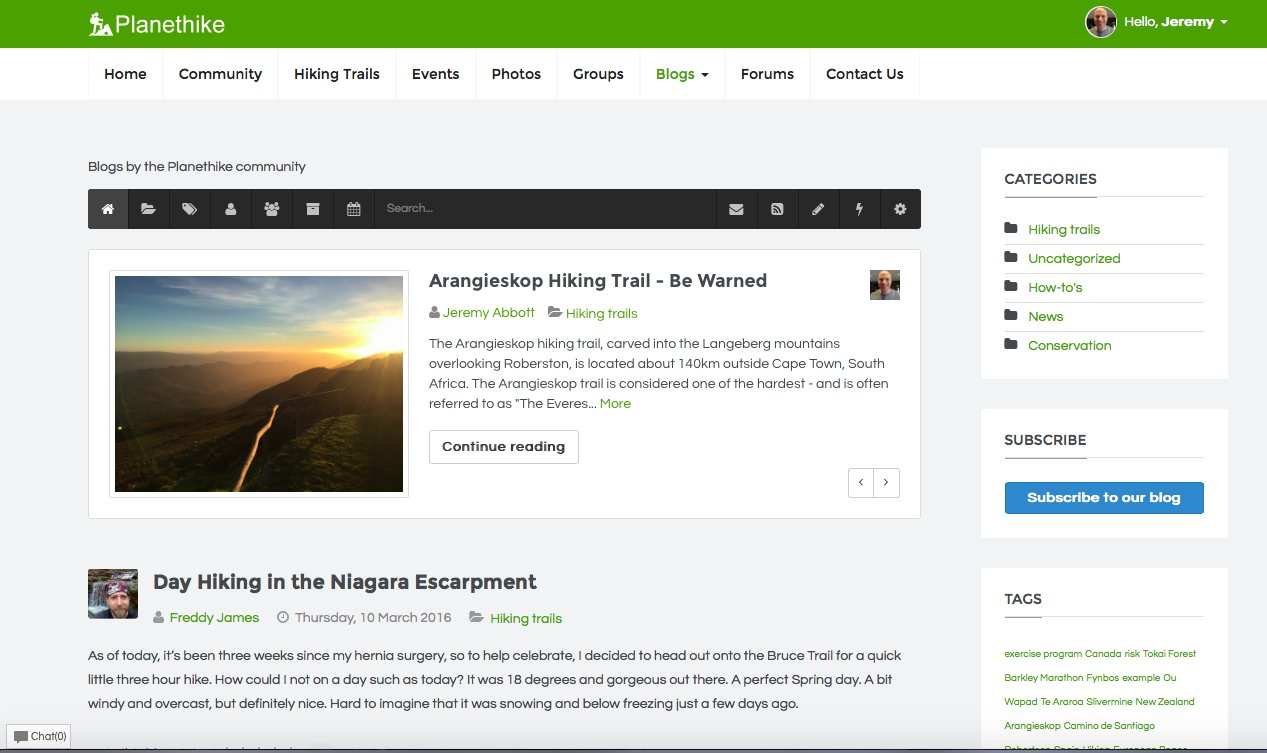
\includegraphics[width=320pt]{slike/planethike1.JPG}}
\hspace{10 pt}
\subfigure[]{\label{fig:b}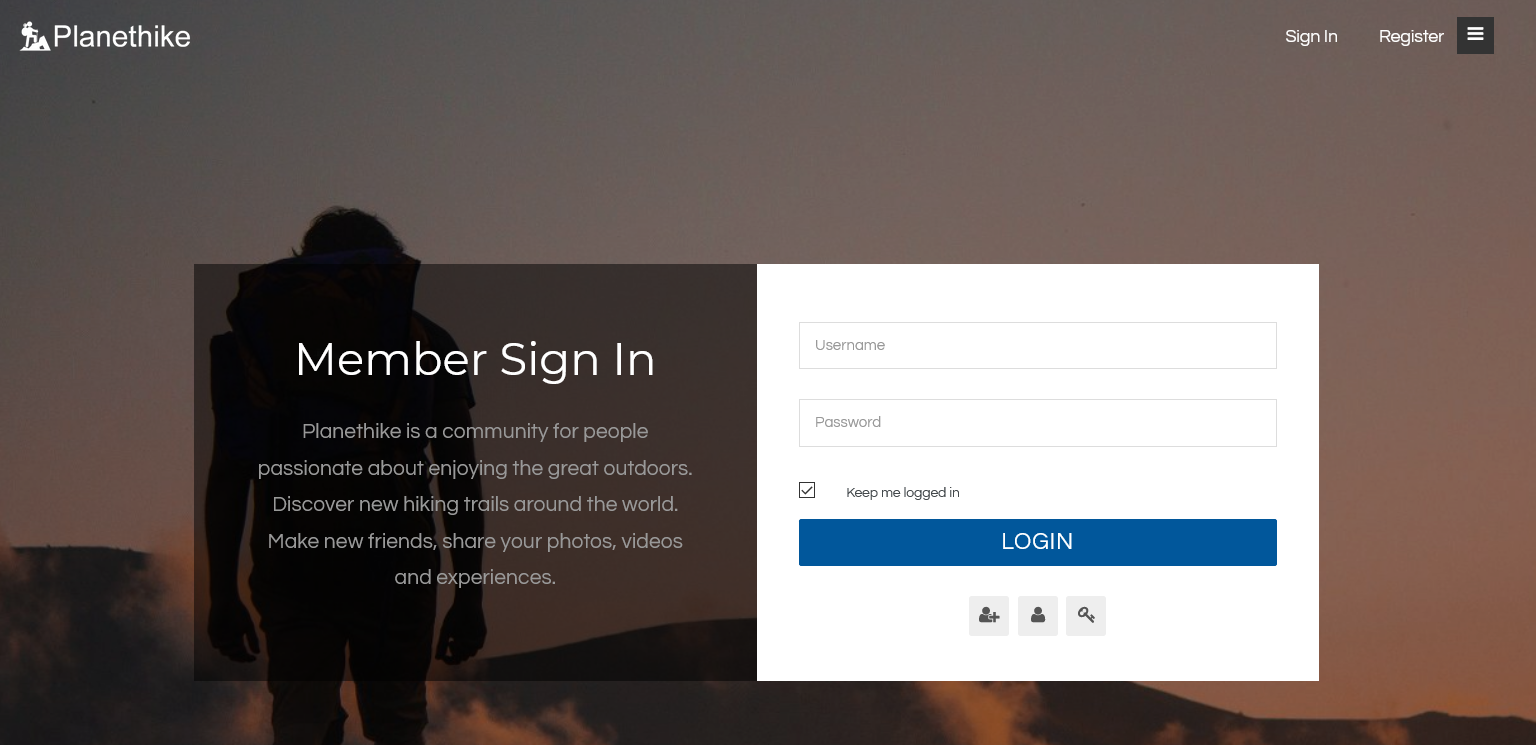
\includegraphics[width=320pt]{slike/planethike2.JPG}}
\hspace{10 pt}
\subfigure[]{\label{fig:c}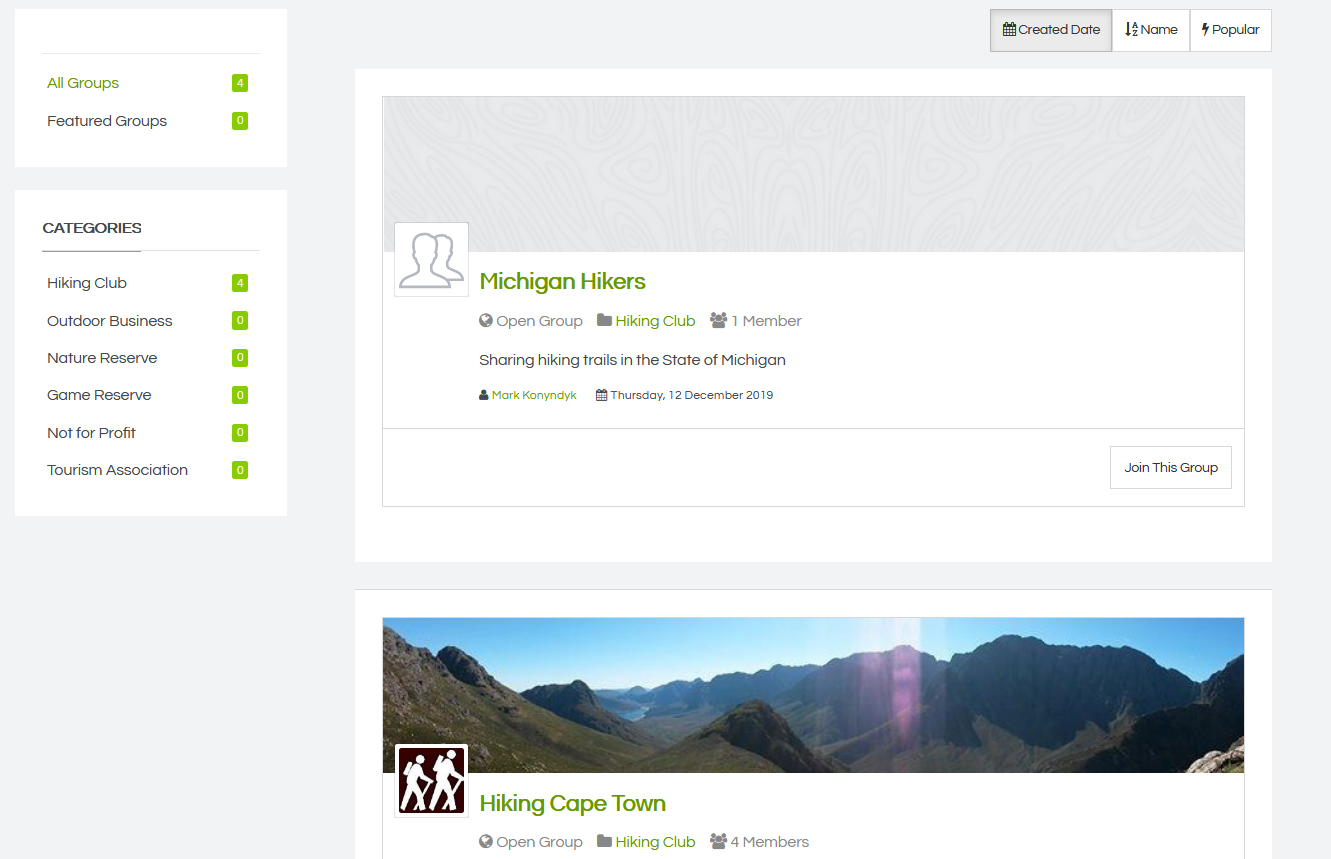
\includegraphics[width=320pt]{slike/planethike3.JPG}}
\caption{Planet hike društvena mreža}
\end{figure}

Potencijalni korisnici ove aplikacije su gotovo svi koji žele planinariti, a pritom se pripremiti za izlet ili podijeliti iskustvo nakon izleta s drugim planinarima. Pristup aplikaciji imaju svi, a korisniku se na izbor daje želi li se registrirati i prijaviti kao registrirani korisnik (hiker) ili želi samo pregledavati aplikaciju bez dodavanja sadržaja kao gost.\vspace{10pt}

\textbf{Gostu} je omogućen pregled i pretraga unaprijed definiranih planinarskih izleta koji su javni, a organizirani su prema geografskom području, trajanju i zahtjevnosti planinarskog izleta. Svaki izlet sadrži informacije o postojanju planinarskih domova i odmorišta s dostupnom infrastrukturom (prenoćište, hrana, pitka voda, struja i dr.) unutar Republike Hrvatske. \vspace{10pt}

Da bi pristupio svim funkcionalnostima aplikacije korisnik se mora registrirati i prijaviti u sustav. Podaci koje korisnik treba unijeti prilikom registracije su:

\begin{packed_item}
			\item \textit{ime}
			\item \textit{prezime}
			\item \textit{korisničko ime}
			\item \textit{lozinka}
			\item \textit{korisnička fotografija}
\end{packed_item}

Nakon uspješne registracije korisnik se nalazi na naslovnoj stranici Planinarskog dnevnika i pregledava vidljivi sadržaj na njoj; slike, događaje, bedževe i izlete. Da bi sadržaj naslovnice bio ispunjen sadržajem korisnik bi trebao dodati prijatelje čiji će se sadržaj pojavljivati. Ostale korisnike moguće je pronaći unosom određenih podataka u tražilicu na kartici \textbf{zajednica}. Kada korisnik uspostavi prijateljstva te kada njegovi prijatelju počnu objavljivati sadržaj on će, radi lakše snalažljivosti, moći filtrirati sadržaj koji mu se prikazuje na naslovnoj stranici. Sadržaj se filtrira prema sljedećim opcijama: 

\begin{packed_item}
			\item \textit {slike}
			\item \textit{događaji}
			\item \textit {bedževi}
			\item \textit{izleti}
\end{packed_item}

\textbf{Registrirani i prijavljeni korisnici} mogu kreirati vlastiti planinarski izlet (javno ili privatno) prema definiranom predlošku koji zahtijeva neke osnovne informacije:

\begin{packed_item}
			\item \textit {odredište}
			\item \textit{planinarski domovi i odmorišta}
			\item \textit{zahtjevnost izleta}
			\item \textit{dužina staze}
			\item \textit{prosječno trajanje izleta}
			\item \textit{opis izleta}
\end{packed_item} 

Pored kreiranja vlastitog planinarskog izleta, registrirani i prijavljeni korisnici mogu ocijeniti planinarski izlet te prijaviti netočne informacije, a prijavu će pregledati \textbf{administrator} ili \textbf{kreator izleta}. Ukoliko korisnik naiđe na izlet koji bi ga mogao zanimati može ga dodati na \textbf{listu željenih izleta} označavanjem ikone pored javnog izleta.
Nakon što korisnik odradi jedan od objavljenih izleta, može zatražiti potvrdu od \textbf{dežurnog planinara}. \vspace{10pt}

Nakon odrađenog niza planinarskih izleta ili stečenog postignuća korisnik može dobiti jedan ili više mogućih \textbf{bedževa} koji su implementirani kao sistem nagrađivanja. Nakon ispunjenog cilja korisnik dobije obavijest da je osvojio bedž te mu se nudi mogućnost da bedž podijeli na svom profilu i naslovnici sa svojim prijateljima. 
\vspace{10pt}

Kako bi se korisnici mogli zajedno sastati na nekom događaju ili izletu omogućena je i funkcija za kreiranje događaja. Korisnik mora biti registriran i prijavljen te odabrati karticu za \textbf{kreiranje događaja}. Važno je da u trenutku kreiranja događaja korisnik ima prijatelje koje bi mogao pozvati na događaj, u suprotnom aplikacija ne dopušta kreiranje događaja. Nakon toga ispunjava predložak koji zahtijeva neke informacije o događaju:

\begin{packed_item}
			\item \textit {naziv }
			\item \textit{datum}
			\item \textit{opis}
			\item \textit{popis pozvanih prijatelja}
\end{packed_item} 

S druge strane, korisnici koji su pozvani na događaj dobivaju prikladnu obavijesti i imaju mogućnost prihvaćanja ili odbijanja poziva. Pozivatelj nakon odgovora dobije obavijest o tome je li pozivnica prihvaćena ili odbijena.
	%\documentclass[12pt]{article}
%
%\title{Specifikacija programske potpore}
%
%\usepackage[slovene]{babel}
%\usepackage[utf8]{inputenc}
%\usepackage{hyperref}
%
%%Meta data
%\hypersetup{
%unicode=true
%}
%
%\begin{document}
\chapter{Specifikacija programske potpore}

\section{Funkcionalni zahtjevi}
\textbf{Dionici:}
\begin{enumerate}
\item Gost (neprijavljeni korisnik)
\item Prijavljeni korisnik
\item Dežurni planinar
\item Administrator
\end{enumerate}
\noindent
\textbf{Aktori i njihovi funkcionalni zahtjevi:}
\begin{enumerate}
%\item [\textbf{Aktori i njihovi funkcionalni zahtjevi:}]
\item \underline{Neprijavljeni korisnik (inicijator) može:}
\begin{enumerate}
\item registrirati se ili se prijaviti
%\item pretražiti registrirane korisnike i vidjeti njihove profile %nismo se dogovorili
\item pretražiti i vidjeti unaprijed definirane planinarske izlete
\end{enumerate}

\item \underline{Prijavljeni korisnik (inicijator) može:}
\begin{enumerate}
\item pretražiti registrirane korisnike i vidjeti njihove profile
\item vidjeti i promijeniti svoj profil (sliku, status, bedževe)
\item pretražiti i vidjeti unaprijed definirane planinarske izlete
\item dodati unaprijed definirane planinarske izlete, planinarske domove i skloništa na popis željenih
\item kreirati vlastiti planinarski izlet prema unaprijed definiranom predlošku
\item kreirani planinarski izlet zadržati privatnim ili ga podijeliti sa svim ostalim korisnicima aplikacije
\item ocjenjivati javno dostupne planinarske izlete
\item prijaviti netočne ili neprecizne informacije javno dostupnih planinarskih izleta
\item kreirati događaj vidljiv na zidu obavijesti
\item pozvati korisnike aplikacije s popisa vlastite planinarske zajednice sa zida obavijesti
\item vidjeti popis prihvaćenih ili odbijenih pozivnica
%\item dvosmjerna komunikacija %chat? ili se nismo dogovorili šta je to
\item vidjeti nove objave korisnika s popisa vlastite planinarske zajednice
\item dodati u arhivu ranije odrađene planinarske izlete
\end{enumerate}

\item \underline{Dežurni planinar (inicijator) može:}
\begin{enumerate}
\item pretražiti registrirane korisnike i vidjeti njihove profile
\item vidjeti i promijeniti svoj profil (sliku, status, bedževe)
\item pretražiti i vidjeti unaprijed definirane planinarske izlete
\item dodati unaprijed definirane planinarske izlete, planinarske domove i skloništa na popis željenih
\item kreirati vlastiti planinarski izlet prema unaprijed definiranom predlošku
\item kreirani planinarski izlet zadržati privatnim ili ga podijeliti sa svim ostalim korisnicima aplikacije
\item ocjenjivati javno dostupne planinarske izlete
\item prijaviti netočne ili neprecizne informacije javno dostupnih planinarskih izleta
\item kreirati ili obrisati vlastiti događaj vidljiv na zidu obavijesti
\item pozvati korisnike aplikacije s popisa vlastite planinarske zajednice na postojeći događaj
\item vidjeti popis prihvaćenih ili odbijenih pozivnica
%\item dvosmjerna komunikacija %chat? piše ko fejsbuk
\item vidjeti nove objave korisnika s popisa vlastite planinarske zajednice
\item dodati u arhivu ranije odrađene planinarske izlete
\item dati registriranom korisniku potvrdu o posjetu planinarskog doma
\end{enumerate}

\item \underline{Administrator (inicijator) može:}
\begin{enumerate}
\item vidjeti popis svih registriranih korisnika i njihovih osobnih podataka
\item brisati korisnike i mijenjati im razinu pristupa aplikaciji
\item brisati tuđe događaje
\item promijeniti informacije javno dostupnom planinarskom izletu
\item dodati ili obrisati planinsku rutu
\item dodijeliti ili oduzeti bilo koji bedž registriranim korisnicima
\end{enumerate}

\item \underline{Baza podataka (sudionik):}
\begin{enumerate}
\item pohranjuje sve podatke o korisnicima i njihovim ovlastima
%\item pohranjuje sve podatke o upitima i njihovim rezultatima %nismo se još dogovorili
\end{enumerate}

\end{enumerate}

	\subsection{Obrasci uporabe}
	
		\subsubsection{Opis obrazaca uporabe}
		
			\noindent \underbar{\textbf{UC01 - Registracija}}
			\begin{packed_item}
				
				\item \textbf{Glavni sudionik: } Gost
				\item  \textbf{Cilj:} Izraditi korisnički račun za pristup društvenoj mreži planinara.
				\item  \textbf{Sudionici:} Baza podataka
				\item  \textbf{Preduvjet:} Korisnik u trenutnoj sesiji nije prijavljen.
				\item  \textbf{Opis osnovnog tijeka:}
				
				\item[] \begin{packed_enum}
					
					\item Korisnik odabire opciju za registraciju na ekranu za prijavu.
					\item Sustav otvara ekran za registraciju.
					\item Korisnik unosi ime, prezime, korisničko ime, lozinku i prenosi sliku s uređaja.
					\item Korisnik pritišće gumb za registraciju.
					\item Sustav provjerava točnost podataka.

					\item Baza podataka provjerava da korisnik s tim korisničkim imenom već ne postoji.
					\item Sustav stvara korisnički račun i preusmjerava korisnika na početnu stranicu.
				\end{packed_enum}
				
				\item  \textbf{Opis mogućih odstupanja:}
				
				\item[] \begin{packed_item}
					
					\item[5.a] Podaci su nepotpuni ili pogrešni. 
					\item[] \begin{packed_enum}
						
						\item Sustav daje korisniku do znanja koji podaci su neispravni.
						\item Sustav ide u korak 3.
						
					\end{packed_enum}
					
					\item[6.a] Korisnik s tim korisničkim imenom već postoji. 
					\item[] \begin{packed_enum}
						
						\item Sustav daje korisniku do znanja da mora koristiti drugo korisničko ime.
						\item Sustav ide u korak 3.
						
					\end{packed_enum}
					
				\end{packed_item}
			\end{packed_item}


			\noindent \underbar{\textbf{UC02 - Pregled tuđeg profila}}
			\begin{packed_item}
				
				\item \textbf{Glavni sudionik: } Korisnik
				\item  \textbf{Cilj:} Vidjeti informacije o nekom drugom korisniku planinaru.
				\item  \textbf{Sudionici:} Baza podataka
				\item  \textbf{Preduvjet:} Korisnik je prijavljen. Ne mora biti prijatelj s dotičnom osobom.
				\item  \textbf{Opis osnovnog tijeka:}
				
				\item[] \begin{packed_enum}
					
					\item Korisnik se nalazi na naslovnici (news feed).
					\item Korisnik pretražuje planinara putem tražilice planinara ili pritišće na njegovu sliku, odnosno ime i prezime, tamo gdje se taj planinar već nalazi na naslovnici.
					\item Baza podataka dohvaća podatke o tom planinaru.
					\item Otvara se profil tog planinara.
					
				\end{packed_enum}
				
				\item  \textbf{Opis mogućih odstupanja:}
				
				\item[] \begin{packed_item}
					
					\item[4.a] Korisnik nije prijatelj s dotičnim planinarom. 
					\item[] \begin{packed_enum}
						
						\item Sustav daje korisniku manje informacija o tom planinaru.
					\end{packed_enum}
						
					
				\end{packed_item}
			\end{packed_item}


			\noindent \underbar{\textbf{UC03 - Filtriranje sadržaja naslovnice}}
			\begin{packed_item}
				
				\item \textbf{Glavni sudionik: } Korisnik
				\item  \textbf{Cilj:} Prikazati samo željene planinarske informacije na naslovnici.
				\item  \textbf{Sudionici:} Baza podataka
				\item  \textbf{Preduvjet:} Korisnik je prijavljen i nalazi se na naslovnici.
				\item  \textbf{Opis osnovnog tijeka:}
				
				\item[] \begin{packed_enum}
					
					\item Korisnik se nalazi na naslovnici (news feed).
					\item Odabire opciju filtriranja sadržaja naslovnice.
					\item Odabire opciju filtriranja - slike, događaji, bedževi ili izleti.
					\item Pritišće gumb za filtriranje odabranog sadržaja.
					\item Na naslovnici se prikazuju samo odabrani sadržaji.
					
				\end{packed_enum}
				
				\item  \textbf{Opis mogućih odstupanja:}
				
				\item[] \begin{packed_item}
					
					\item[3.a] Ne postoji niti jedan sadržaj koji zadovoljava filter. 
					\item[] \begin{packed_enum}
						
						\item Sustav obavještava korisnika primjerenom obaviješću.
					\end{packed_enum}
					
					
				\end{packed_item}
			\end{packed_item}
		
		\noindent \underbar{\textbf{UC04 - Prikaz vlastitog profila}}
		\begin{packed_item}
			
			\item \textbf{Glavni sudionik: } Korisnik
			\item  \textbf{Cilj:} Vidjeti vlastite informacije dostupne na ovoj društvenoj planinarskoj mreži.
			\item  \textbf{Sudionici:} Baza podataka
			\item  \textbf{Preduvjet:} Korisnik je prijavljen.
			\item  \textbf{Opis osnovnog tijeka:}
			
			\item[] \begin{packed_enum}
				
				\item Korisnik se nalazi na bilo kojoj kartici (naslovnica, planinarske staze, ...)
				\item Korisnik pritišće na karticu profil.
				\item Baza podataka dohvaća podatke o tom planinaru.
				\item Otvara se vlastiti profil planinara.
				
			\end{packed_enum}
		\end{packed_item}
	
		\noindent \underbar{\textbf{UC05 - Prikaz naslovnice}}
		\begin{packed_item}
			
			\item \textbf{Glavni sudionik: } Korisnik
			\item  \textbf{Cilj:} Vidjeti aktualne informacije i novosti vezane uz prijatelje planinare.
			\item  \textbf{Sudionici:} Baza podataka
			\item  \textbf{Preduvjet:} Korisnik je prijavljen. 
			\item  \textbf{Opis osnovnog tijeka:}
			
			\item[] \begin{packed_enum}
				
				\item Korisnik se nalazi na bilo kojoj kartici u aplikaciji(profil, planinarski izleti, ...).
				\item Pritišće na karticu Naslovnica.
				\item Baza podataka pohvaća podatke o novostima vezanima uz prijatelje dotičnog planinara.
				\item Korisnik pregledava naslovnicu.
				
			\end{packed_enum}
			
			\item  \textbf{Opis mogućih odstupanja:}
			
			\item[] \begin{packed_item}
				
				\item[3.a] Korisnik nema prijatelja. 
				\item[] \begin{packed_enum}
					
					\item Sustav to daje korisniku do znanja te ga potiče da uspostavi neka prijateljstva.
				\end{packed_enum}
			
				\item[3.b] Korisnik ima prijatelje, ali nitko od njih nije aktivan pa se na naslovnici nema što prikazati. 
				\item[] \begin{packed_enum}
					
					\item Sustav obavještava korisnika da kod njegovih prijatelja nema nikakvih novosti te ga motivira da uspostavi nova prijateljstva.
				\end{packed_enum}
				
				
			\end{packed_item}
		\end{packed_item}
		
		\noindent \underbar{\textbf{UC06 - Dodavanje prijatelja}}
		\begin{packed_item}
			
			\item \textbf{Glavni sudionik: } Korisnik
			\item  \textbf{Cilj:} Povezivanje dvaju korisnika te mogućnost interakcije i pregleda sadržaja koji je vidljiv samo prijateljima.
			\item  \textbf{Sudionici:} Baza podataka
			\item  \textbf{Preduvjet:} Korisnik je prijavljen i nije prijatelj s korisnikom kojeg želi dodati.
			\item  \textbf{Opis osnovnog tijeka:}
			
			\item[] \begin{packed_enum}
				
				\item Korisnik se nalazi na naslovnici (news feed).
					\item Korisnik pretražuje planinara putem tražilice planinara ili pritišće na njegovu sliku odnosno ime i prezime tamo gdje se taj planinar već nalazi na naslovnici.
					\item Baza podataka dohvaća podatke o tom planinaru.
					\item Otvara se profil tog planinara.
					\item Korisnik pritišće gumb za slanje zahtjeva za prijateljstvo.
					\item Planinaru se šalje zahtjev za prijateljstvo od korisnika.
					\item Gumb za slanje zahtjeva za prijateljstvo mijenja izgled i obavještava korisnika da je zahtjev za prijateljstvo poslan.
				
			\end{packed_enum}
			
			\item  \textbf{Opis mogućih odstupanja:}
			
			\item[] \begin{packed_item}
				
				\item[3.a] Planinar je prethodno korisniku poslao zahtjev za prijateljstvom. 
				\item[] \begin{packed_enum}
					
					\item Gumb za slanje zahtjeva za prijateljstvo mijenja se u gumb za prihvaćanje zahtjeva za prijateljstvo.
				\end{packed_enum}
					
			\end{packed_item}
		\end{packed_item}
		
		\noindent \underbar{\textbf{UC07 - Pretraživanje planinara}}
		\begin{packed_item}
			
			\item \textbf{Glavni sudionik: } Korisnik
			\item  \textbf{Cilj:} Pronalazak planinara na zajednici pomoću poznatih informacija.
			\item  \textbf{Sudionici:} Baza podataka
			\item  \textbf{Preduvjet:} Korisnik je prijavljen i nalazi se na kartici "Zajednica".
			\item  \textbf{Opis osnovnog tijeka:}
			
			\item[] \begin{packed_enum}
				
				\item Korisnik se nalazi na kartici "Zajednica".
				\item Korisnik pretražuje planinara putem tražilice planinara.
				\item Podaci uneseni u tražilicu uspoređuju se s podacima iz baze podataka te se pronalaze profili planinara koji se podudaraju s unesenim informacijama.
				\item Korisniku se prikazuju pronađeni planinari.
				
			\end{packed_enum}
			
			\item  \textbf{Opis mogućih odstupanja:}
			
			\item[] \begin{packed_item}
					
					\item[3.a] Ne postoji niti jedan planinar koji zadovoljava unesene podatke za pretraživanje.
					\item[] \begin{packed_enum}
						
						\item Sustav obaviještava korisnika primjerenom obaviješću.
					\end{packed_enum}
				
				
			\end{packed_item}
		\end{packed_item}
		
		\noindent \underbar{\textbf{UC08 - Ocjenjivanje javno dostupnih izleta}}
		\begin{packed_item}
			
			\item \textbf{Glavni sudionik: } Korisnik
			\item  \textbf{Cilj:} Ocjenjivanje izleta kako bi se drugim korisnicima olakšao odabir, a kreatoru izleta dala povratna informacija.
			\item  \textbf{Sudionici:} Baza podataka
			\item  \textbf{Preduvjet:} Korisnik je prijavljen i izlet je javno dostupan.
			\item  \textbf{Opis osnovnog tijeka:}
			
			\item[] \begin{packed_enum}
				
				\item Korisnik se nalazi na kartici planinarskog izleta.
					\item Korisnik pritiskom na zvjezdicu odabire koliko zvjezdica (od 1 do 5) želi dati izletu.
					\item Ocjena izleta ažurira se u bazi podataka.
					\item Korisnik sada umjesto praznih zvjezdica vidi koliko je zvjezdica dao javnom izletu. 
				
			\end{packed_enum}
			
			\item  \textbf{Opis mogućih odstupanja:}
			
			\item[] \begin{packed_item}
					
					\item[3.a] Korisnik je već ocijenio izlet.
					\item[] \begin{packed_enum}
						
						\item Sustav omogućuje korisniku da promijeni svoju ocjenu.
					\end{packed_enum}
				
				
			\end{packed_item}
		\end{packed_item}

		\noindent \underbar{\textbf{UC09 - Kreiranje izleta}}
		\begin{packed_item}
			
			\item \textbf{Glavni sudionik: } Korisnik
			\item  \textbf{Cilj:} Kreirati izlet
			\item  \textbf{Sudionici:} Baza podataka
			\item  \textbf{Preduvjet:} Korisnik je prijavljen i nalazi se na naslovnici ili pregledava izlete ili kreira novi događaj.
			\item  \textbf{Opis osnovnog tijeka:}
			
			\item[] \begin{packed_enum}
				
				\item Korisnik se nalazi na naslovnici (news feed) ili pregledava izlete ili kreira novi događaj.
				\item Korisnik odabire karticu "Kreiraj izlet".
				\item Otvara se stranica na kojoj se nalazi predložak za kreiranje izleta.
				\item Korisnik popunjava predložak.
				\item Korisnik odabire opciju "Kreiraj".
				\item Baza podataka sprema podatke.
				\item Korisnik završava s kreiranjem te je vraćen na prethodnu stranicu s koje je proslijeđen na kreiranje.
				
			\end{packed_enum}
			
			\item  \textbf{Opis mogućih odstupanja:}
			
			\item[] \begin{packed_item}
				
				\item[4.a] Korisnik ispuni predložak, ali ne odabere opciju "Kreiraj". 
				\item[] \begin{packed_enum}
					
					\item Sustav obavještava korisnika primjerenom obaviješću.
				\end{packed_enum}
				
				
			\end{packed_item}
		\end{packed_item}
		
		
		\noindent \underbar{\textbf{UC10 - Dodavanje izleta na popis željenih}}
		\begin{packed_item}
			
			\item \textbf{Glavni sudionik: } Korisnik
			\item  \textbf{Cilj:} Dodati izlet na popis željenih.
			\item  \textbf{Sudionici:} Baza podataka
			\item  \textbf{Preduvjet:} Korisnik je prijavljen.
			\item  \textbf{Opis osnovnog tijeka:}
			
			\item[] \begin{packed_enum}
				
				\item Korisnik pregledava javne planinarske izlete.
				\item Nad željenim izletom korisnik označuje ikonu za dodavanje u favorite.
				\item Baza podataka sprema podatke.
			
			\end{packed_enum}
		\end{packed_item}
		
		
		
		\noindent \underbar{\textbf{UC11 - Prijava netočnih/nepreciznih informacija}}
		\begin{packed_item}
			
			\item \textbf{Glavni sudionik: } Korisnik
			\item  \textbf{Cilj:} Prijaviti netočne/neprecizne informacije.
			\item  \textbf{Sudionici:} Baza podataka, Admin
			\item  \textbf{Preduvjet:} Korisnik je prijavljen.
			\item  \textbf{Opis osnovnog tijeka:}
			
			\item[] \begin{packed_enum}
				
				\item Korisnik pregledava javne planinarske izlete.
				\item Korisnik na izletu odabire opciju "Prijavi".
				\item Otvara se oblačić u koji korisnik piše razlog prijave.
				\item Korisnik odabire opciju "Pošalji prijavu".
				\item Baza podataka sprema podatke.
				\item Prijavu zaprima korisnik koji je napravio izlet ili admin ako je izlet predefiniran.
				
			\end{packed_enum}
			
			\item  \textbf{Opis mogućih odstupanja:}
			
			\item[] \begin{packed_item}
				
				\item[3.a] Korisnik napiše razlog prijave, ali ne odabere opciju "Pošalji prijavu". 
				\item[] \begin{packed_enum}
					
					\item Sustav obavještava korisnika primjerenom obaviješću.
				\end{packed_enum}
				
				
			\end{packed_item}
		\end{packed_item}
		
		
		\noindent \underbar{\textbf{UC12 - Kreiranje događaja}}
		\begin{packed_item}
			
			\item \textbf{Glavni sudionik: } Korisnik
			\item  \textbf{Cilj:} Kreirati događaj.
			\item  \textbf{Sudionici:} Baza podataka
			\item  \textbf{Preduvjet:} Korisnik je prijavljen i nalazi se na naslovnici.
			\item  \textbf{Opis osnovnog tijeka:}
			
			\item[] \begin{packed_enum}
				
				\item Korisnik se nalazi na naslovnici.
				\item Korisnik odabire karticu "Kreiraj događaj".
				\item Otvara se stranica na kojoj se nalazi predložak za kreiranje izleta.
				\item Korisnik popunjava predložak.
				\item Korisnik odabire prijatelje iz liste prijatelja .
				\item Korisnik odabire opciju "Kreiraj".
				\item Baza podataka sprema podatke.
				
			\end{packed_enum}
			
			\item  \textbf{Opis mogućih odstupanja:}
			
			\item[] \begin{packed_item}
				
				\item[4.a] Korisnik ispuni predložak, ali ne odabere opciju "Kreiraj". 
				\item[] \begin{packed_enum}
					
					\item Sustav obavještava korisnika primjerenom obaviješću.
				\end{packed_enum}
			
				\item[5.a] Korisnik nije odabrao niti jednog prijatelja. 
				\item[] \begin{packed_enum}
				
					\item Sustav obavještava korisnika da mora odabrati barem jednog prijatelja.
				\end{packed_enum}
			
				\item[5.b] Korisnik nema prijatelja. 
				\item[] \begin{packed_enum}
				
					\item Sustav to korisniku daje do znanja te ga potiče da uspostavi neka prijateljstva.
				\end{packed_enum}
				
				
			\end{packed_item}
		\end{packed_item}
		
		
		
		\noindent \underbar{\textbf{UC13 - Prihvaćanje/odbijanje događaja}}
		\begin{packed_item}
			
			\item \textbf{Glavni sudionik: } Korisnik
			\item  \textbf{Cilj:} Prihvatiti ili odbiti pozivnicu na događaj.
			\item  \textbf{Sudionici:} Baza podataka
			\item  \textbf{Preduvjet:} Korisnik je prijavljen i pozvan na događaj.
			\item  \textbf{Opis osnovnog tijeka:}
			
			\item[] \begin{packed_enum}
				
				\item Korisnik dobije obavijest da je pozvan na događaj.
				\item Korisnik odabire opciju "Prihvati" ili "Odbij".
				\item Baza podataka sprema podatke.
				\item Korisnik koji je poslao pozivnicu dobiva obavijest o tome je li pozivnica prihvaćena.
				
			\end{packed_enum}
		\end{packed_item}
		
		
		\noindent \underbar{\textbf{UC14 - Prihvaćanje/odbijanje dežurnih planinara}}
		\begin{packed_item}
			
			\item \textbf{Glavni sudionik: } Administrator
			\item  \textbf{Cilj:} Prihvatiti ili odbiti registraciju za dežurnog planinara.
			\item  \textbf{Sudionici:} Baza podataka, Korisnik
			\item  \textbf{Preduvjet:} Korisnik je prijavljen i dodijeljena su mu prava administratora.
			\item  \textbf{Opis osnovnog tijeka:}
			
			\item[] \begin{packed_enum}
				
				\item Administrator dobije obavijest o registraciji.
				\item Administrator otvvara popis registracija.
				\item Odabire opciju "Prihvati" ili "Odbij".
				\item Korisnik dobiva obavijest o tome je li registracija prihvaćena.
				\item Baza podataka sprema podatke.
				
			\end{packed_enum}
		\end{packed_item}
		
		
		
		\noindent \underbar{\textbf{UC15 - Dobivanje bedža}}
		\begin{packed_item}
			
			\item \textbf{Glavni sudionik: } Korisnik
			\item  \textbf{Cilj:} Dobivanje bedža.
			\item  \textbf{Sudionici:} Baza podataka
			\item  \textbf{Preduvjet:} Korisnik je prijavljen i postigao je određeni cilj.
			\item  \textbf{Opis osnovnog tijeka:}
			
			\item[] \begin{packed_enum}
				
				\item Korisnik postiže određeni cilj (Prijeđeni kilometri, nadmorska visina,...).
				\item Korisnik prima obavijest da je dobio bedž.
				\item Baza podataka sprema podatke.
				
			\end{packed_enum}
		\end{packed_item}

				\noindent \underbar{\textbf{UC16 - Objavljivanje bedža}}
		\begin{packed_item}
			
			\item \textbf{Glavni sudionik: } Korisnik
			\item  \textbf{Cilj:} Podijeliti vijest osvojenog bedža s prijateljima.
			\item  \textbf{Sudionici:} Baza podataka	%nisam siguran
			\item  \textbf{Preduvjet:} Korisnik je upravo osvojio bedž.
			\item  \textbf{Opis osnovnog tijeka:}
			
			\item[] \begin{packed_enum}
				
				\item Sustav otvara skočni prozor za objavu bedža.
				\item Korisnik pritišće gumb za objavu bedža.
				\item Sustav prikazuje objavu korisniku i svim prijateljima korisnika.
				
			\end{packed_enum}
			
			\item  \textbf{Opis mogućih odstupanja:}
			
			\item[] \begin{packed_item}
				
				\item[2.a] Korisnik pritišće gumb za odustajanje od objave.
				\item[] \begin{packed_enum}
					
					\item Sustav zatvara skočni prozor.
					
				\end{packed_enum}
				
			\end{packed_item}
		\end{packed_item}
	
	
		\noindent \underbar{\textbf{UC17 - Pregled javno dostupnih izleta}}
		\begin{packed_item}
			
			\item \textbf{Glavni sudionik: } Korisnik i gost
			\item  \textbf{Cilj:} Pregledavanje javno dostupnih izleta.
			\item  \textbf{Sudionici:} Baza podataka
			\item  \textbf{Preduvjet:} Korisnik je prijavljen kao gost ili planinar.
			\item  \textbf{Opis osnovnog tijeka:}
			
			\item[] \begin{packed_enum}
				
				\item Korisnik odabire karticu "Planinarski izleti".
				\item Baza podataka izbacuje sve javno dostupne planinarske izlete.
				\item Korisniku se prikazuju svi javno dostupni planinarski izleti.
				
			\end{packed_enum}
		\end{packed_item}
		
		
		
		\noindent \underbar{\textbf{UC18 - Pretraga javnih planinarskih izleta}}
		\begin{packed_item}
			
			\item \textbf{Glavni sudionik: } Korisnik i gost
			\item  \textbf{Cilj:} Pretraživanje i filtriranje javnih planinarskih izleta.
			\item  \textbf{Sudionici:} Baza podataka
			\item  \textbf{Preduvjet:} Korisnik je prijavljen kao gost ili kao planinar.
			\item  \textbf{Opis osnovnog tijeka:}
			
			\item[] \begin{packed_enum}
				
				\item Korisnik odabire karticu "Planinarski izleti".
				\item Baza podataka izbacuje sve javno dostupne planinarske izlete.
				\item Korisniku se prikazuju svi javno dostupni planinarski izleti.
				\item Korisnik odabire opciju za pretraživanje javnih planinarskih izleta.
				\item Korisni upisuje naziv javnog planinarskog izleta.
				\item Korisnik stavlja određene filtere za sužavanje pretrage.
				\item Baza podataka izbacuje sve javne planinarske izlete koji spadaju pod navedenu kategoriju.
				\item Korisniku se prikazuju svi javno dostupni planinarski izleti sortirani po kriteriju korisnika.
				
			\end{packed_enum}
			
			\item	\textbf{Opis mogućih odstupanja:}
			
			\item[] \begin{packed_item}
				
				\item[8.a] Korisniku se ne prikazuje nijedan planinarski izlet jer nijedan ne spada u navedenu kategoriju.
				\item[] \begin{packed_enum}
					
					\item Korisnik mijenja kriterije ili odustaje od pretrage javnih planinarskih izleta.
				\end{packed_enum}
				
			\end{packed_item}
		\end{packed_item}
		
		
		
		\noindent \underbar{\textbf{UC19 - Prijava u aplikaciju}}
		\begin{packed_item}
			
			\item \textbf{Glavni sudionik: } Korisnik
			\item  \textbf{Cilj:} Pristupanje planinarskom dnevniku s pogodnostima prijavljenog planinara.
			\item  \textbf{Sudionici:} Baza podataka
			\item  \textbf{Preduvjet:} Registracija za planinarski dnevnik.
			\item  \textbf{Opis osnovnog tijeka:}
			
			\item[] \begin{packed_enum}
				
				\item Korisnik unosi svoje korisničko ime i zaporku s kojom se registrirao u zasebne obrazce.
				\item Baza podataka prima podatke koje je unio korisnik.
				\item Baza podataka provjerava točnost podataka.
				\item Baza podataka vraća povratnu informaciju o točnosti unesenih podataka sa strane korisnika.
				\item Korisnik je prijavljen u aplikaciju planinarskog dnevnika s pogodnostima prijavljenog planinara.
				
			\end{packed_enum}
			
			\item	\textbf{Opis mogućih odstupanja:}
			
			\item[] \begin{packed_item}
				
				\item[5.a] Korisnik nije prijavljen te je vraćen na stranicu prijave.
				\item[] \begin{packed_enum}
					
					\item Sustav mu javlja da su mu podaci netočni te da ponovno upiše svoje podatke.
				\end{packed_enum}
				
			\end{packed_item}
		\end{packed_item}
		
		
		
		\noindent \underbar{\textbf{UC20 - Nastavi kao gost}}
		\begin{packed_item}
			
			\item \textbf{Glavni sudionik: } Korisnik
			\item  \textbf{Cilj:} Pristupanje planinarskom dnevniku bez pogodnosti prijavljenog planinara.
			\item  \textbf{Sudionici:} Baza podataka
			\item  \textbf{Preduvjet:} -
			\item  \textbf{Opis osnovnog tijeka:}
			
			\item[] \begin{packed_enum}
				
				\item Od ponuđenih opcija korisnik bira "Nastavi kao gost".
				\item Baza podataka mu daje privremeni nadimak.
				\item Korisnik je prijavljen u aplikaciju planinarskog dnevnika bez pogodnosti prijavljenog planinara.
				
			\end{packed_enum}
		\end{packed_item}
		
		
		
		\noindent \underbar{\textbf{UC21 - Pregled osobnih podataka}}
		\begin{packed_item}
			
			\item \textbf{Glavni sudionik: } Korisnik
			\item  \textbf{Cilj:} Pregled osobnih podataka planinara.
			\item  \textbf{Sudionici:} Baza podataka
			\item  \textbf{Preduvjet:} Korisnik je registriran i prijavljen u aplikaciju planinarskog dnevnika.
			\item  \textbf{Opis osnovnog tijeka:}
			
			\item[] \begin{packed_enum}
				
				\item Korisnik je prijavljen u aplikaciju.
				\item Korisnik odabire opciju "Osobni podaci".
				\item Baza podataka prikuplja informacije o planinaru.
				\item Baza podataka šalje informacije o planinaru.
				\item Korisniku se prikazuju njegovi vlastiti podaci o računu.
				
			\end{packed_enum}
		\end{packed_item}
		
		
		
		\noindent \underbar{\textbf{UC22 - Promjena osobnih podataka}}
		\begin{packed_item}
			
			\item \textbf{Glavni sudionik: } Korisnik
			\item  \textbf{Cilj:} Mijenjanje vlastitih podataka planinara.
			\item  \textbf{Sudionici:} Baza podataka
			\item  \textbf{Preduvjet:} Korisnik je registriran i prijavljen u aplikaciju planinarskog dnevnika.
			\item  \textbf{Opis osnovnog tijeka:}
			
			\item[] \begin{packed_enum}
				
				\item Korisnik je prijavljen u aplikaciju.
				\item Korisnik odabire opciju "Osobni podaci".
				\item Baza podataka prikuplja informacije o planinaru.
				\item Baza podataka šalje informacije o planinaru.
				\item Korisniku se prikazuju njegovi vlastiti podaci o računu.
				\item Korisnik odabire koji od podataka želi promijeniti.
				\item Korisnik unosi promjene.
				\item Baza podataka prima nove podatke.
				\item Korisniku se prikazuju ažurirani vlastiti podaci.
				
			\end{packed_enum}
			
			\item	\textbf{Opis mogućih odstupanja:}
			
			\item[] \begin{packed_item}
				
				\item[9.a] Korisnik je unio nove podatke koji su već zauzeti od strane nekog drugog planinara u sustavu.
				\item[] \begin{packed_enum}
					
					\item Aplikacija ga obavještava o tome.
					\item Korisnik je vraćen na prijašnju stranicu gdje mu je označeno koji se podaci nisu uspjeli ažurirati.
				\end{packed_enum}
				
			\end{packed_item}
		\end{packed_item}
		
		
		
		\noindent \underbar{\textbf{UC23 - Završetak i zapisivanje korisnikova uspjeha}}
		\begin{packed_item}
			
			\item \textbf{Glavni sudionik: } Korisnik i dežurni planinar
			\item  \textbf{Cilj:} Zapisivanje korisnikova uspjeha u završavanju planinarskog izleta.
			\item  \textbf{Sudionici:} Baza podataka
			\item  \textbf{Preduvjet:} Korisnik je registriran, dežurni planinar je registriran i dodijeljena mu je titula dežurnog planinara od strane administratora.
			\item  \textbf{Opis osnovnog tijeka:}
			
			\item[] \begin{packed_enum}
				
				\item Korisnik završetkom svojeg planinarskog izleta dolazi do dežurnog planinara u planinarskom domu.
				\item Korisnik daje svoje podatke dežurnom planinaru koji te podatke sprema u svoju arhivu.
				\item Dežurni planinar ažurira podatke zapisanih korisnika u bazi podataka zapisujući da su odradili planinarski izlet na kojem je on dežuran.
				\item Baza podataka se ažurira
				
			\end{packed_enum}
		\end{packed_item}
		
		
		
		\noindent \underbar{\textbf{UC24 - Registracija dežurnog planinara}}
		\begin{packed_item}
			
			\item \textbf{Glavni sudionik: } Korisnik i administrator
			\item  \textbf{Cilj:} Obavljanje registracije za planinara koji želi dobiti titulu dežurnog planinara za neki planinarski izlet.
			\item  \textbf{Sudionici:} Baza podataka
			\item  \textbf{Preduvjet:} Korisnik je registriran kao planinar, administrator ima privilegije administratora.
			\item  \textbf{Opis osnovnog tijeka:}
			
			\item[] \begin{packed_enum}
				
				\item Obični korisnik aplikacije šalje zahtjev kako bi postao dežurni planinar za određeni planinarski izlet.
				\item Baza podataka prima zahtjev.
				\item Zathjev se prosljeđuje administratoru.
				\item Administrator proučava zahtjev te odlučuje hoće li planinar dobiti titulu dežurnog planinara.
				\item Baza podataka se ažurira.
				\item Planinar dobiva titulu dežurnog planinara te novo korisničko sučelje za obavljanje posla dežurnog planinara.
				
			\end{packed_enum}
			
			\item	\textbf{Opis mogućih odstupanja:}
			
			\item[] \begin{packed_item}
				
				\item[6.a] Planinar je odbijen i ne dobiva titulu dežurnog planinara.
				\item[] \begin{packed_enum}
					
					\item Planinar ponovno šalje zahtjev ili nastavlja koristiti aplikaciju bez titule dežurnog. 
				\end{packed_enum}
				
			\end{packed_item}
		\end{packed_item}
		
		
		
		\noindent \underbar{\textbf{UC25 - Naknadno dodavanje odrađenih izleta}}
		\begin{packed_item}
			
			\item \textbf{Glavni sudionik: } Korisnik 
			\item  \textbf{Cilj:} Naknadno dodati svoje odrađene izlete u arhivu.
			\item  \textbf{Sudionici:} Baza podataka
			\item  \textbf{Preduvjet:} Korisnik je registriran kao planinar, korisnik je prijavljen u sustav.
			\item  \textbf{Opis osnovnog tijeka:}
			
			\item[] \begin{packed_enum}
				
				\item Korisnik odabire opciju "Planinarski izleti".
				\item Korisniku se prikazuju svi javni planinarski izleti.
				\item Korisnik odabire planinarski izlet.
				\item Od ponuđenih opcija (ocjenjivanje izleta, prijava netočnih informacija, itd.) odabire opciju za spremanje izleta u arhivu odrađenih.
				\item Planinarski izlet je označen kao odrađen te je spremljen u korisnikovu arhivu koja je izolirana od ostalih podataka kako se izlet ne bi ubrajao u napredak za korisnikove bedževe.
				
			\end{packed_enum}
		\end{packed_item}
		
		
		
		\noindent \underbar{\textbf{UC26 - Brisanje korisničkog računa}}
		\begin{packed_item}
			
			\item \textbf{Glavni sudionik: } Korisnik 
			\item  \textbf{Cilj:} Brisanje računa korisnika planinarskog dnevnika.
			\item  \textbf{Sudionici:} Baza podataka
			\item  \textbf{Preduvjet:} Korisnik je registriran i prijavljen u aplikaciju planinarskog dnevnika.
			\item  \textbf{Opis osnovnog tijeka:}
			
			\item[] \begin{packed_enum}
				
				\item Korisnik odabire opciju "Osobni podaci".
				\item Korisniku se prikazuju vlastiti podaci u sustavu.
				\item Korisnik odabire opciju "Izbriši moj račun".
				\item Korisnikov račun se briše iz baze podataka.
				\item Korisniku se prikazuje stranica za registraciju i prijavu u aplikaciju planinarskog dnevnika.
				
			\end{packed_enum}
		\end{packed_item}
		
		
		
		\noindent \underbar{\textbf{UC27 - Pregled korisnika}}
		\begin{packed_item}
			
			\item \textbf{Glavni sudionik: } Administrator 
			\item  \textbf{Cilj:} Pregledavanje podataka korisnika aplikacije planinarskog dnevnika.
			\item  \textbf{Sudionici:} Baza podataka
			\item  \textbf{Preduvjet:} Korisnik je registran, prijavljen i ima titulu administratora.
			\item  \textbf{Opis osnovnog tijeka:}
			
			\item[] \begin{packed_enum}
				
				\item Administrator odabire opciju "Pregled korisnika".
				\item Administratoru se prikazuje lista svih registriranih korisnika.
				
			\end{packed_enum}
		\end{packed_item}
		
		
		
		\noindent \underbar{\textbf{UC28 - Brisanje korisnika}}
		\begin{packed_item}
			
			\item \textbf{Glavni sudionik: } Administrator 
			\item  \textbf{Cilj:} Izvanredno brisanje korisnika iz sustava od strane administratora.
			\item  \textbf{Sudionici:} Baza podataka
			\item  \textbf{Preduvjet:} Korisnik je registriran, prijavljen i ima titulu administratora.
			\item  \textbf{Opis osnovnog tijeka:}
			
			\item[] \begin{packed_enum}
				
				\item Administrator odabire opciju "Pregled korisnika".
				\item Administratoru se prikazuje lista svih registriranih korisnika.
				\item Administrator odabire korisnika kojeg želi obrisati.
				\item Podaci o korisniku su izbrisani iz baze podataka.
				
			\end{packed_enum}
		\end{packed_item}
	
	
	
		\noindent \underbar{\textbf{UC29 - Prikaz zajednice}}
		\begin{packed_item}
			
			\item \textbf{Glavni sudionik: } Korisnik 
			\item  \textbf{Cilj:} Prikazivanje kartice "Zajednica".
			\item  \textbf{Sudionici:} Baza podataka
			\item  \textbf{Preduvjet:} Korisnik je registriran i prijavljen.
			\item  \textbf{Opis osnovnog tijeka:}
			
			\item[] \begin{packed_enum}
				
				\item Korisnik odabire opciju "Zajednica".
				\item Baza podataka pregledava sve prijatelje od korisnika.
				\item Korisniku se prikazuje kartica "Zajednica".
				
				
			\end{packed_enum}
		\end{packed_item}
	
	
	
		\noindent \underbar{\textbf{UC30 - Brisanje izleta}}
		\begin{packed_item}
			
			\item \textbf{Glavni sudionik: } Administrator
			\item  \textbf{Cilj:} Brisanje izleta iz baze podataka.
			\item  \textbf{Sudionici:} Baza podataka
			\item  \textbf{Preduvjet:} Korisnik je registriran i prijavljen te ima titulu administratora.
			\item  \textbf{Opis osnovnog tijeka:}
			
			\item[] \begin{packed_enum}
				
				\item Administrator odabire opciju "Planinarski izleti".
				\item Administrator odabire planinarski izlet.
				\item Administrator odabire opciju "Brisanje izleta".
				\item Izlet se briše iz baze podataka.
				
				
			\end{packed_enum}
		\end{packed_item}
	
	
	
		\noindent \underbar{\textbf{UC31 - Promjena izleta}}
		\begin{packed_item}
			
			\item \textbf{Glavni sudionik: } Administrator
			\item  \textbf{Cilj:} Promjena detalja o planinarskom izletu.
			\item  \textbf{Sudionici:} Baza podataka
			\item  \textbf{Preduvjet:} Korisnik je registriran, prijavljen te ima titulu administratora.
			\item  \textbf{Opis osnovnog tijeka:}
			
			\item[] \begin{packed_enum}
				
				\item Administrator odabire opciju "Planinarski izleti".
				\item Administrator odabire planinarski izlet.
				\item Administrator odabire opciju "Promjena izleta".
				\item Administrator unosi podatke koje želi promijeniti.
				\item Baza podataka se ažurira s novim podacima.
				
				
			\end{packed_enum}
		\end{packed_item}
	
	
		
		\subsubsection{Dijagrami obrazaca uporabe}
		
			\begin{figure}[H]
				\centering
				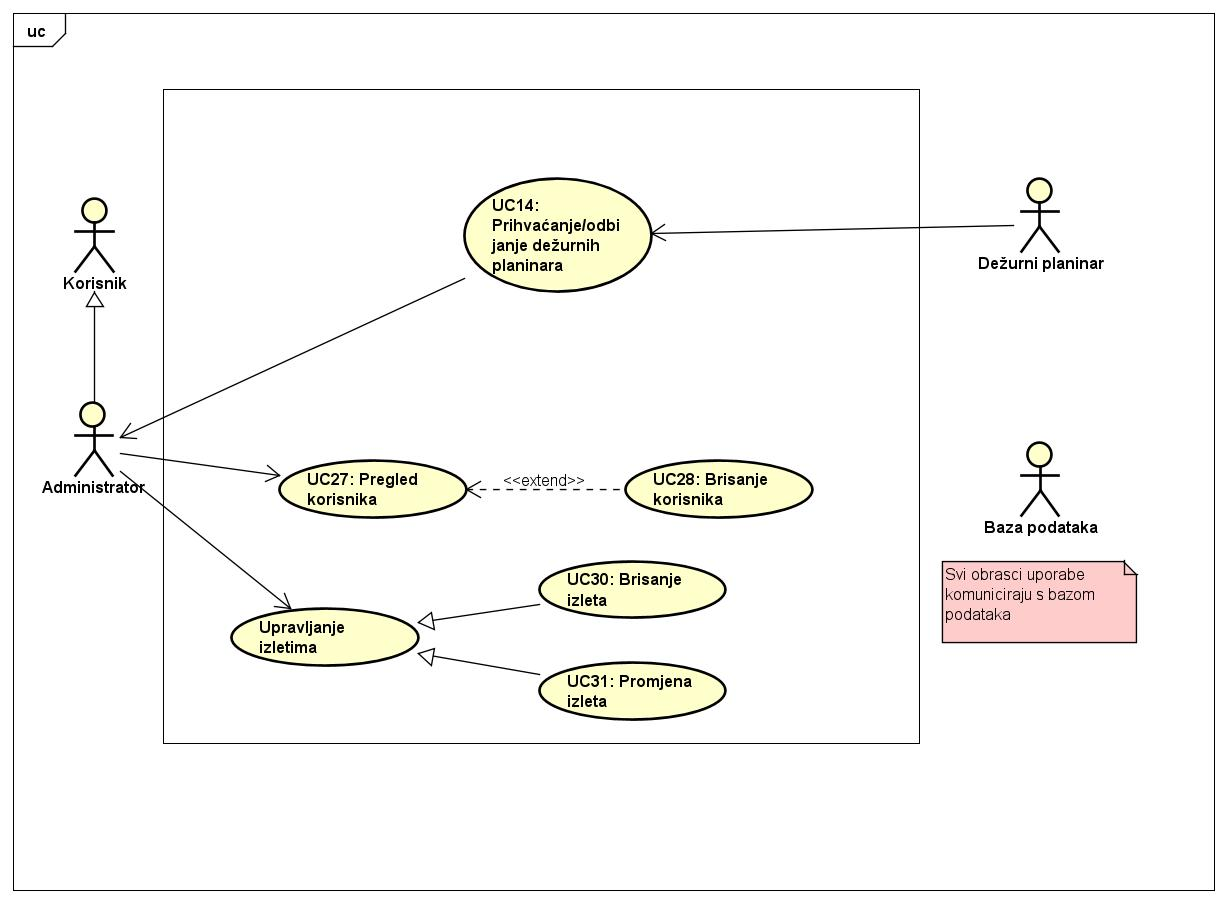
\includegraphics[width=0.9\textwidth]{slike/UC-Administrator.jpg}
				\caption{Dijagram obrasca uporabe, funkcionalnosti administratora}
				\label{fig:mesh1}
			\end{figure}
			
			\vspace{10mm}
			
			\begin{figure}[H]
				\centering
				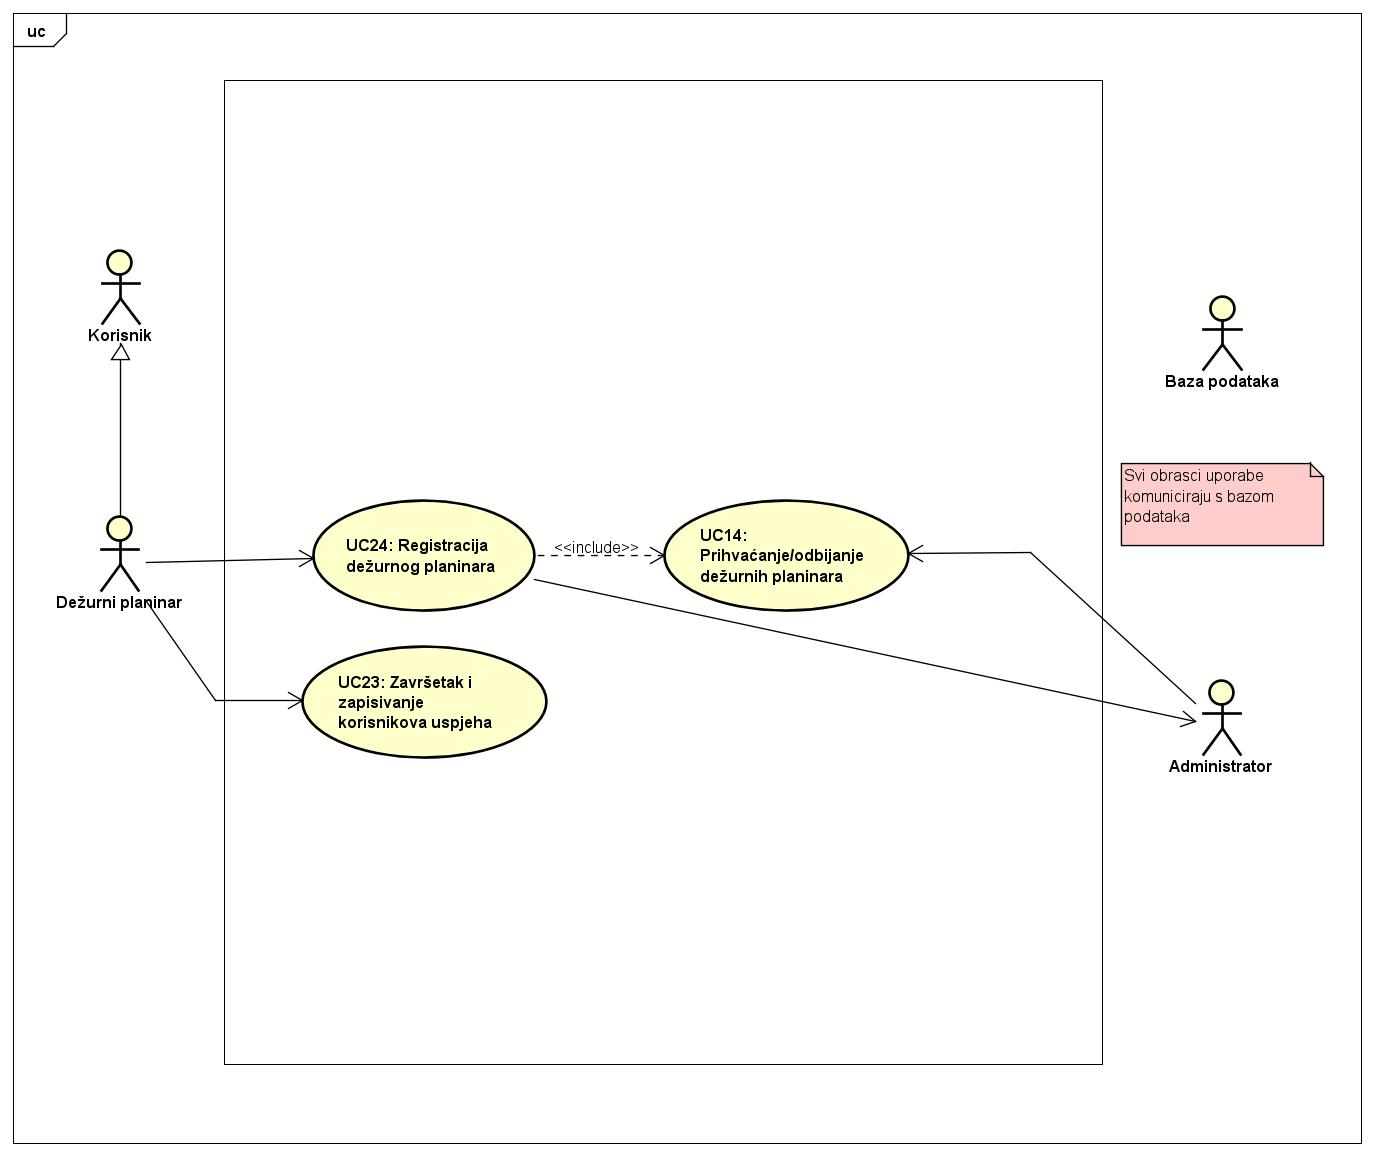
\includegraphics[width=0.9\textwidth]{slike/UC-Dezurni_planinar.jpg}
				\caption{Dijagram obrasca uporabe, funkcionalnosti  dežurnog planinara}
				\label{fig:mesh2}
			\end{figure}
			
			\begin{figure}[H]
				\centering
				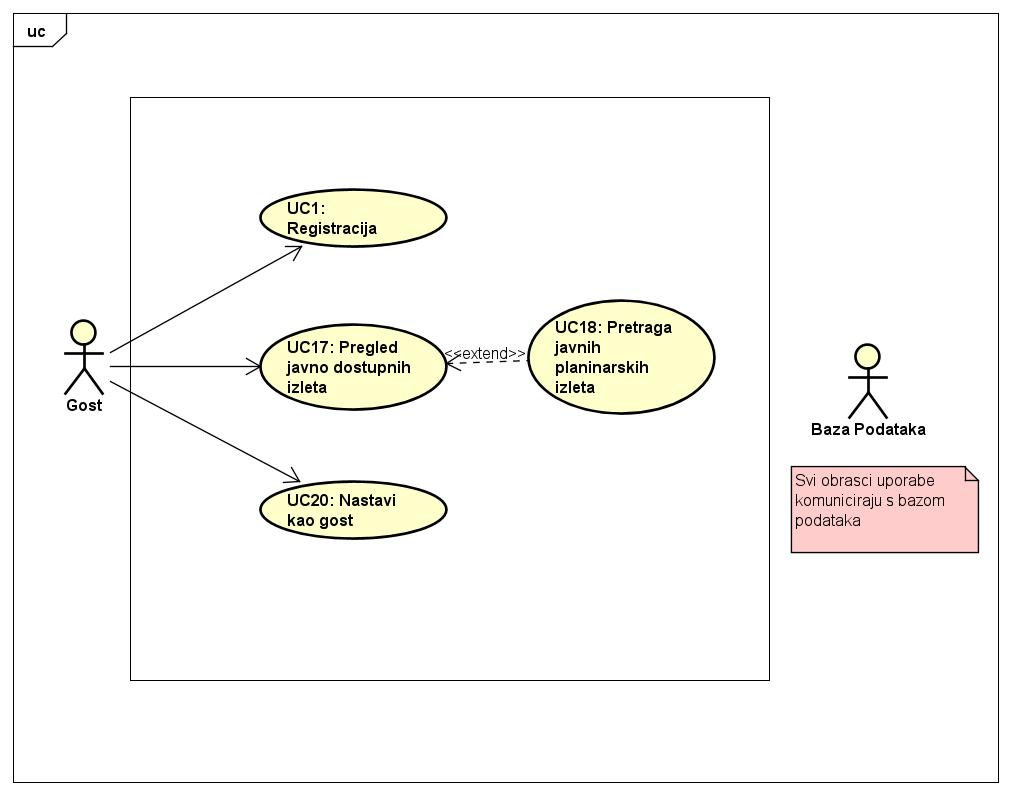
\includegraphics[width=0.9\textwidth]{slike/UC-Gost.jpg}
				\caption{Dijagram obrasca uporabe, funkcionalnosti gosta}
				\label{fig:mesh3}
			\end{figure}
		
			\begin{figure}[H]
				\centering
				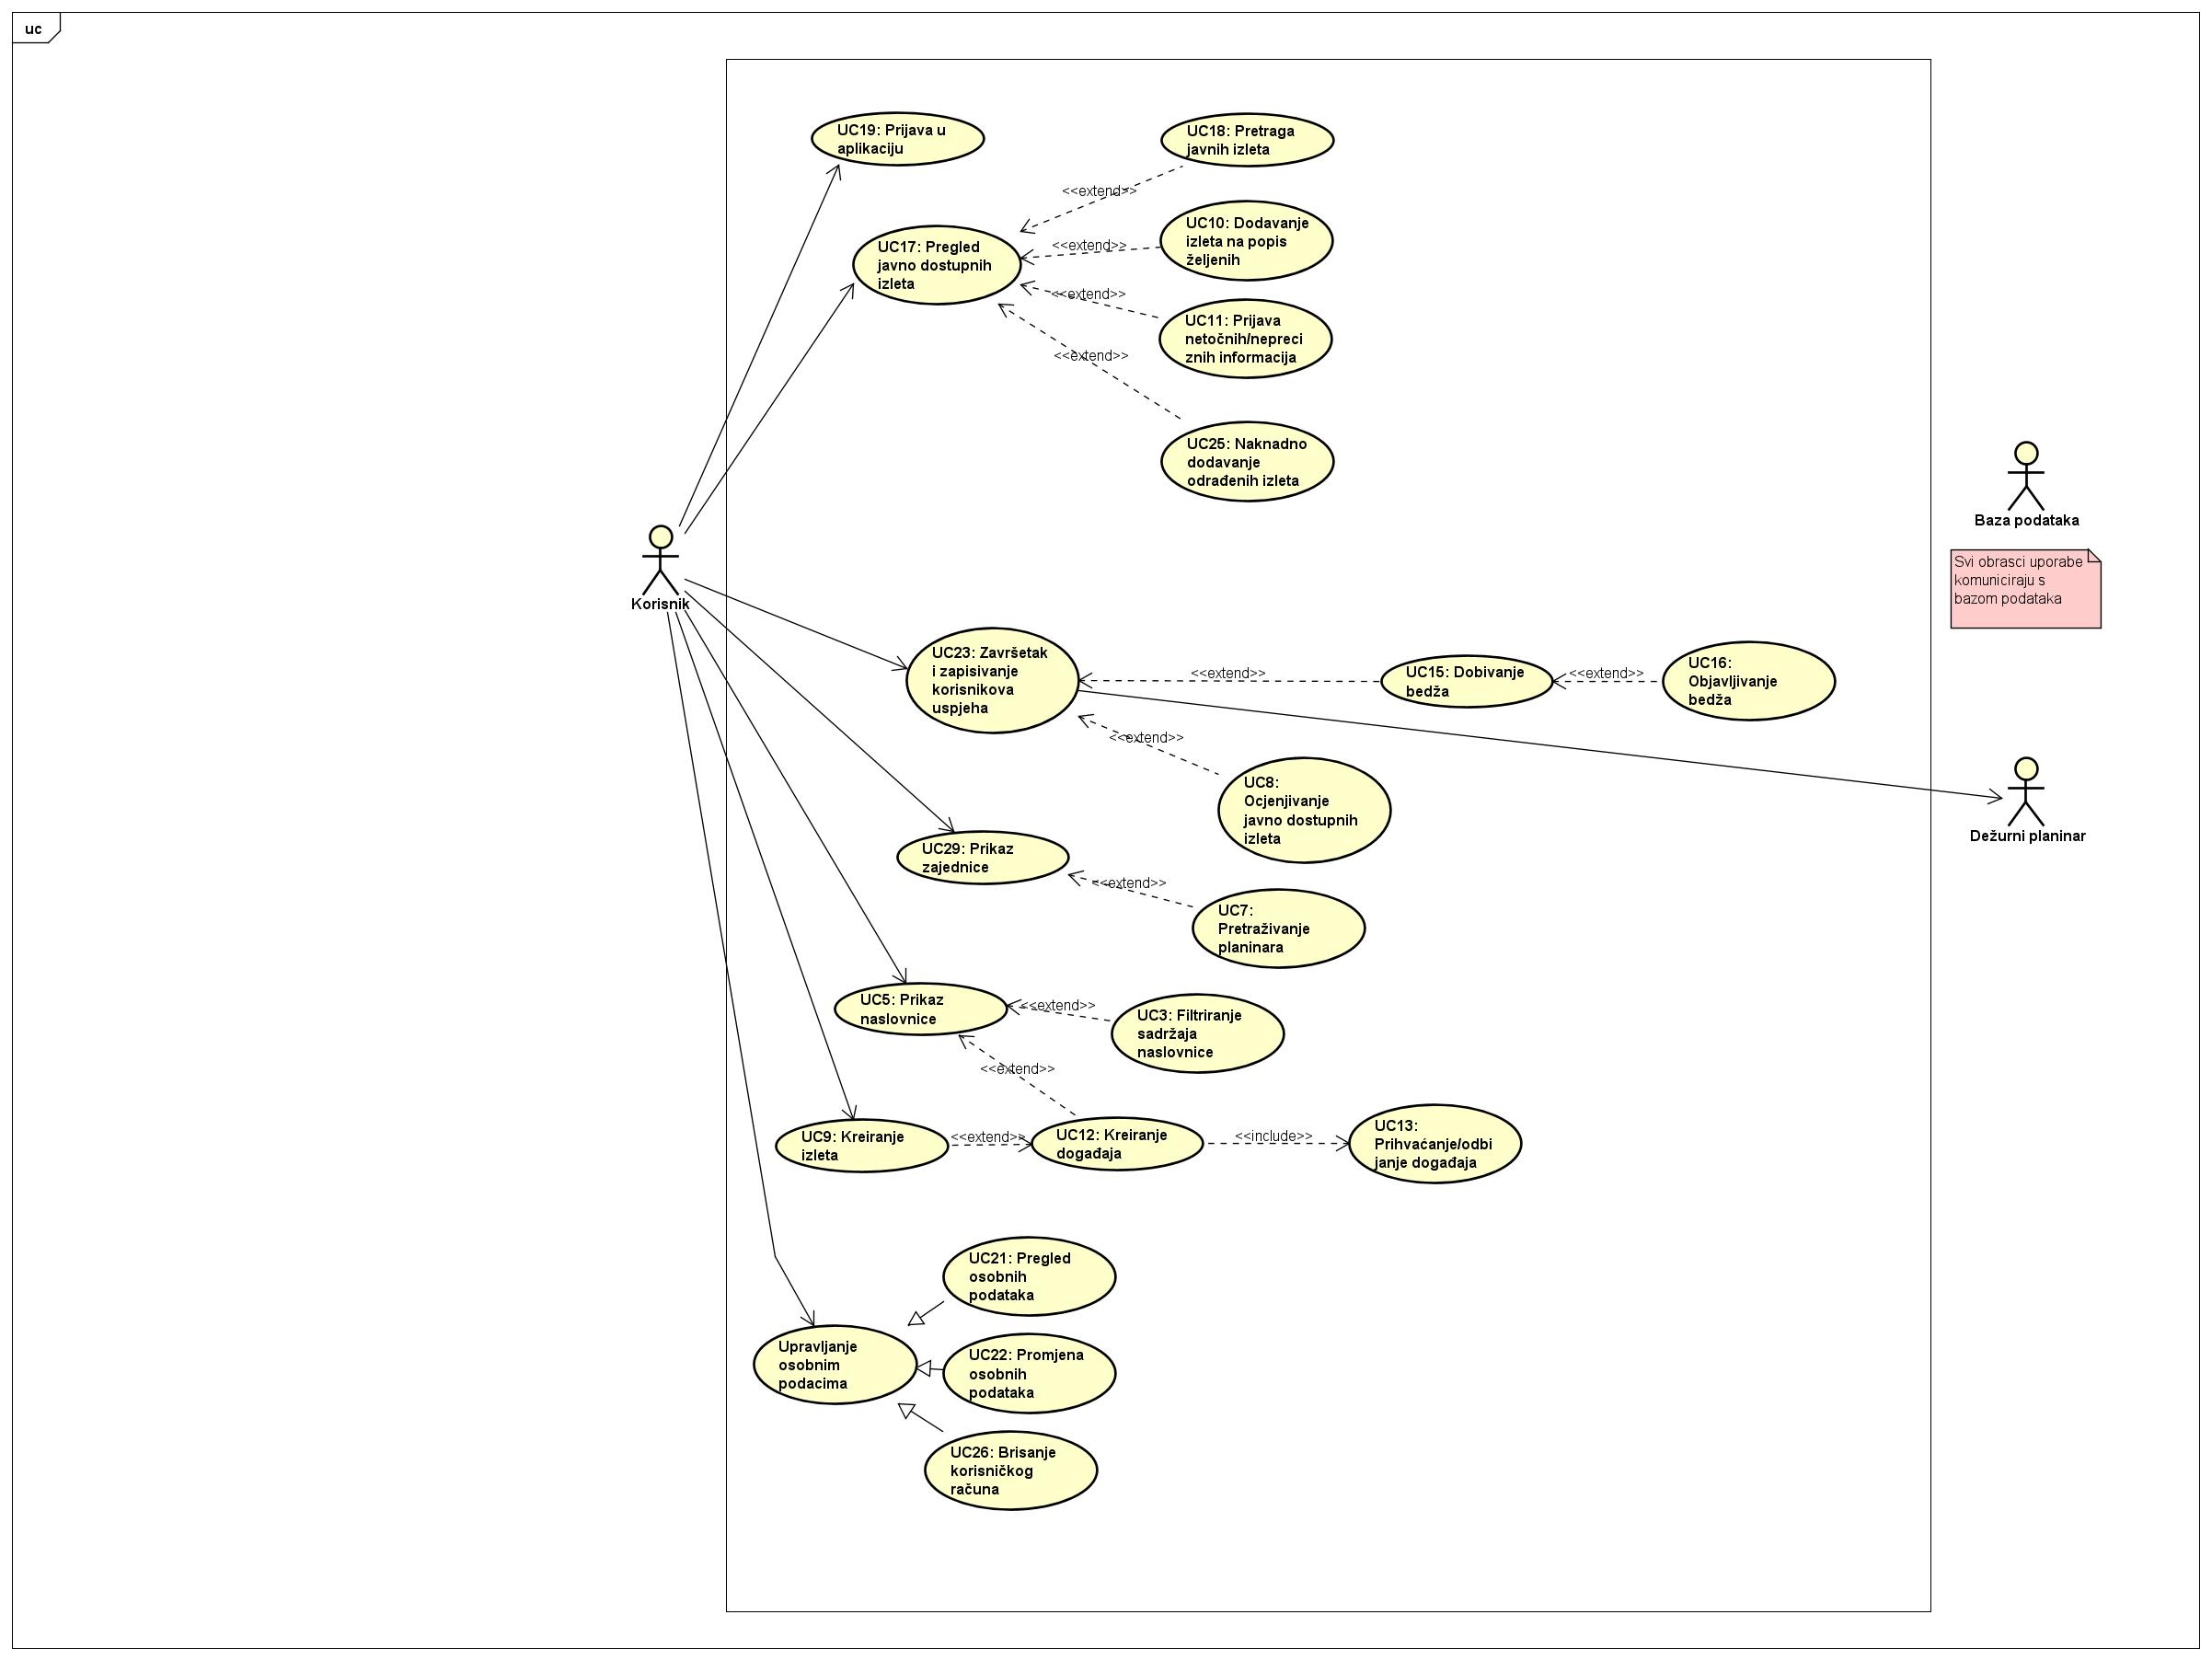
\includegraphics[width=0.9\textwidth]{slike/UC-Korisnik.jpg}
				\caption{Dijagram obrasca uporabe, funkcionalnosti korisnika}
				\label{fig:mesh4}
			\end{figure}
\newpage
	
	
		\subsection{Sekvencijski dijagrami}
		
				\textbf{ Obrazac uporabe 09 - Kreiranje izleta}\\
		
Korisnik je prijavljen i nalazi se na naslovnici ili pregledava izlete ili kreira novi događaj. Korisnik odabire opciju kreiranja izleta. Aplikacija planinarskog dnevnika šalje zahtjev bazi podataka za predložak za kreiranje novog izleta. Baza podataka vraća predložak te aplikacija korisniku prikazuje predložak. Korisnik unosi podatke novog izleta. Korisnik odabire ili kreiranje novog izleta gdje se baza ažurira, vraća potvrdu o uspjehu aplikaciji te aplikacija prikazuje uspjeh korisniku ili odabire opciju za odustajanje od kreiranja izleta te je vraćen na prethodnu stranicu.

		
		
		
				\begin{figure}[H]
					\centering
						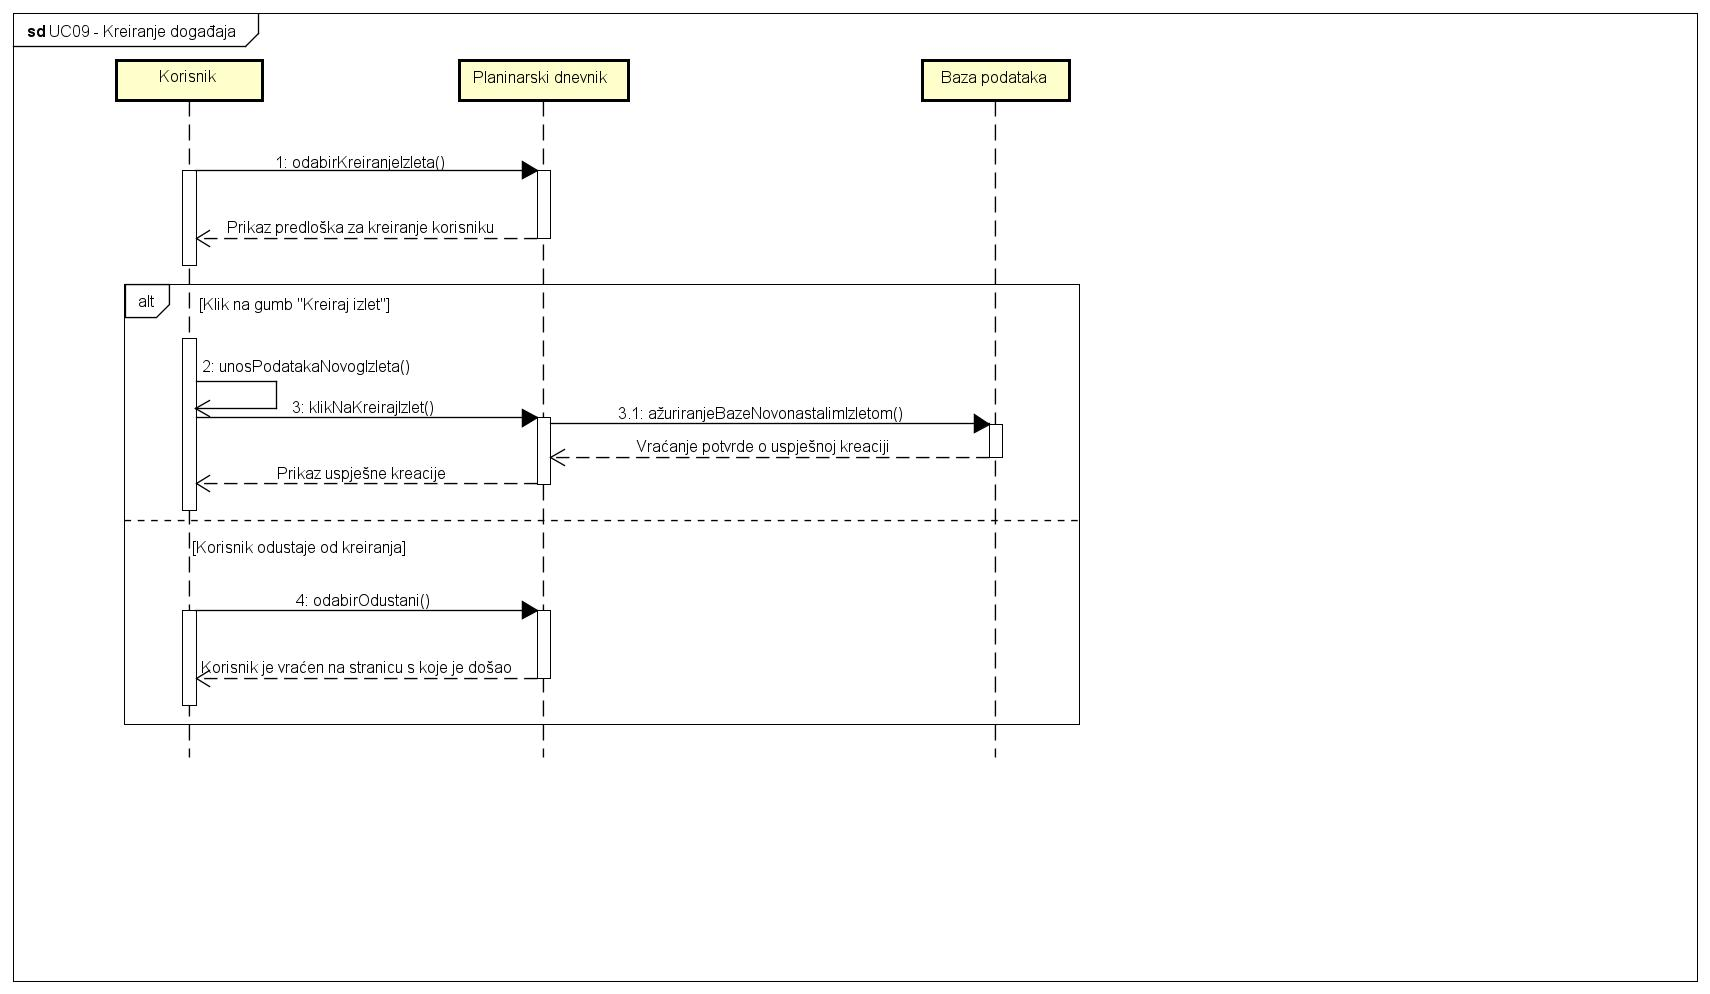
\includegraphics[width=0.9\textwidth]{slike/UC09-Kreiranje_izleta.jpg}
					\caption{Sekvencijski dijagram za UC09}
						\label{fig:mesh5}
				\end{figure}
				
\newpage
			
				\textbf{ Obrazac uporabe 18 - Pretraživanje javnih izleta}\\
				
Korisnik odabire karticu "Planinarski izleti". Planinarski dnevnik prikazuje karticu korisniku. Korisnik odabire opciju pretraživanja javnih planinarski izleta. Web-aplikacija vraća predložak za pretraživanje. Korisnik unosi podatke te klikne na gumb za pretraživanje. Web-aplikacija šalje zahtjev bazi za ispis svih planinarskih izleta koji odgovaraju kriteriju korisnika. Web-aplikacija prikazuje sve planinarske izlete koji odgovaraju korisnikovom kriteriju. Ako se korisniku ne prikazuje nijedan izlet, ponovno unosi podatke i pretražuje ili odustaje od pretrage te je vraćen na karticu "Planinarski izleti".
				
				
				
				\begin{figure}[H]
					\centering
					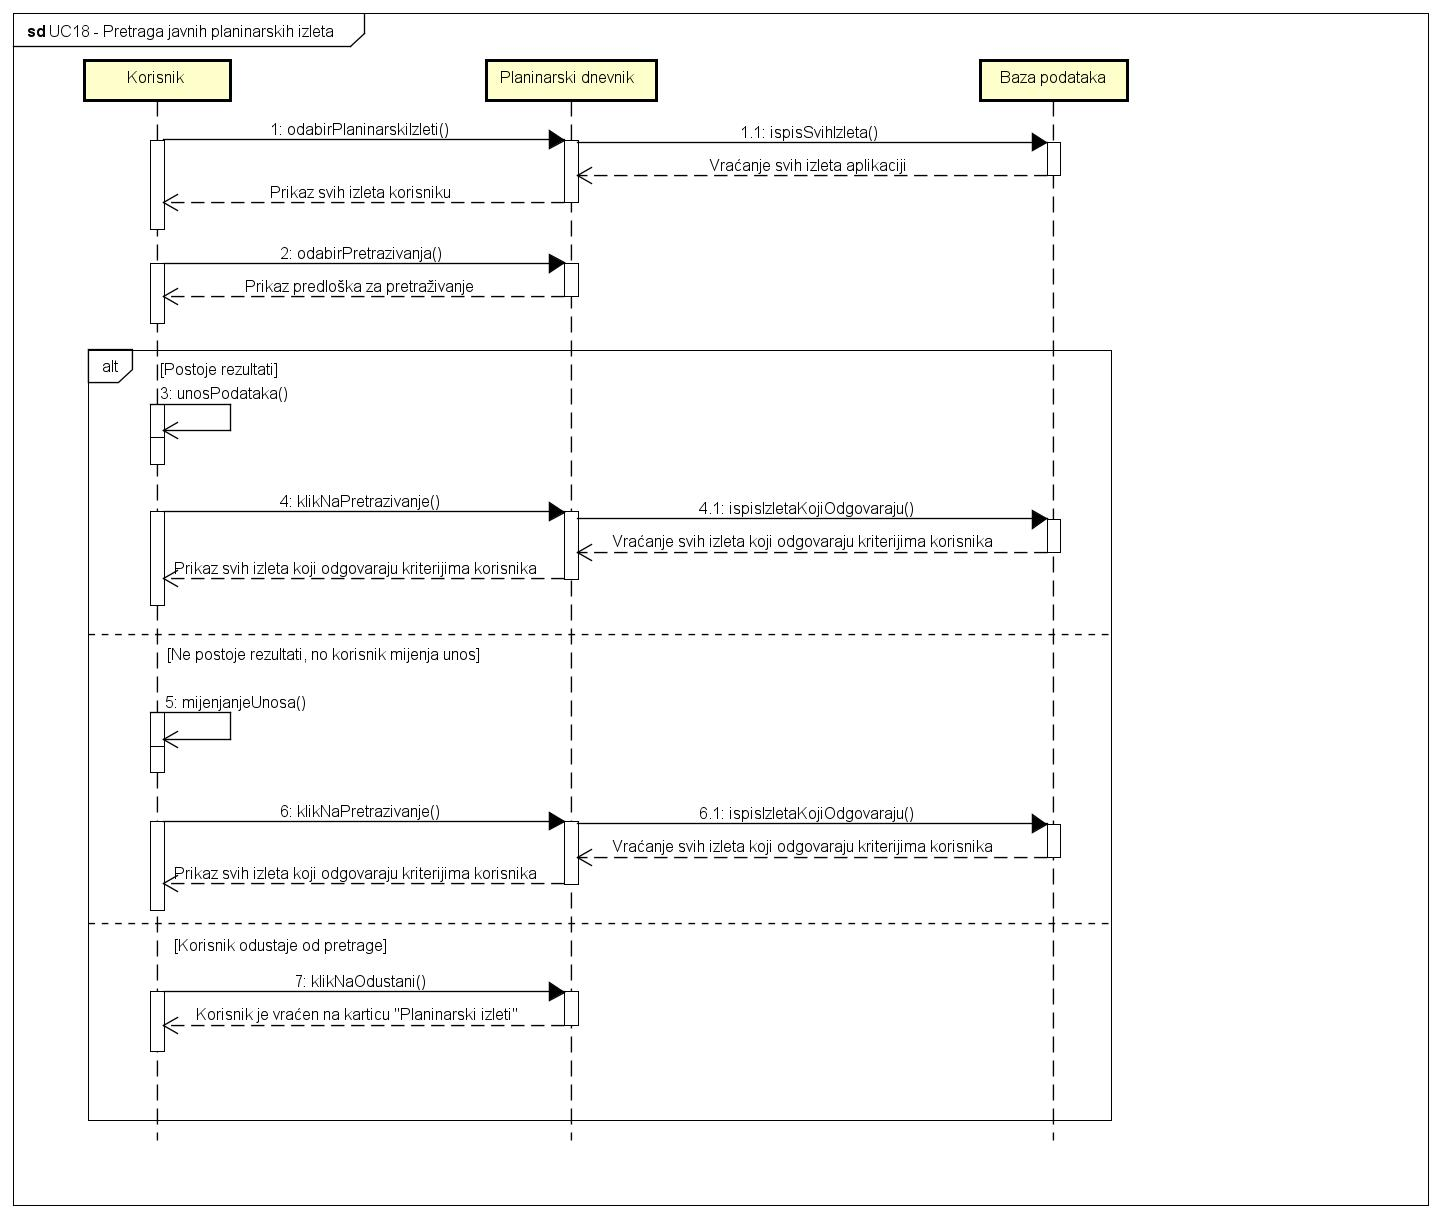
\includegraphics[width=0.9\textwidth]{slike/UC18-Pretraga_javnih_izleta.jpg}
					\caption{Sekvencijski dijagram za UC18}
					\label{fig:mesh6}
				\end{figure}

\newpage
				
				\textbf{ Obrazac uporabe 19 - Prijava u aplikaciju}\\
				
Korisnik se nalazi na stranici za prijavu i unosi svoje podatke za prijavu. Korisnik pritišće gumb za prijavu i šalje podatke koje baza zaprima te provjerava njihovu točnost. Zatim baza podataka daje povratnu informaciju o točnosti podataka nakon čega je korisnik ili prijavljen u aplikaciju (podatci su ispravni) ili je ponovno vraćen na stranicu za prijavu uz prikladnu obavijest (podatci su neispravni).
				
				
				\begin{figure}[H]
					\centering
						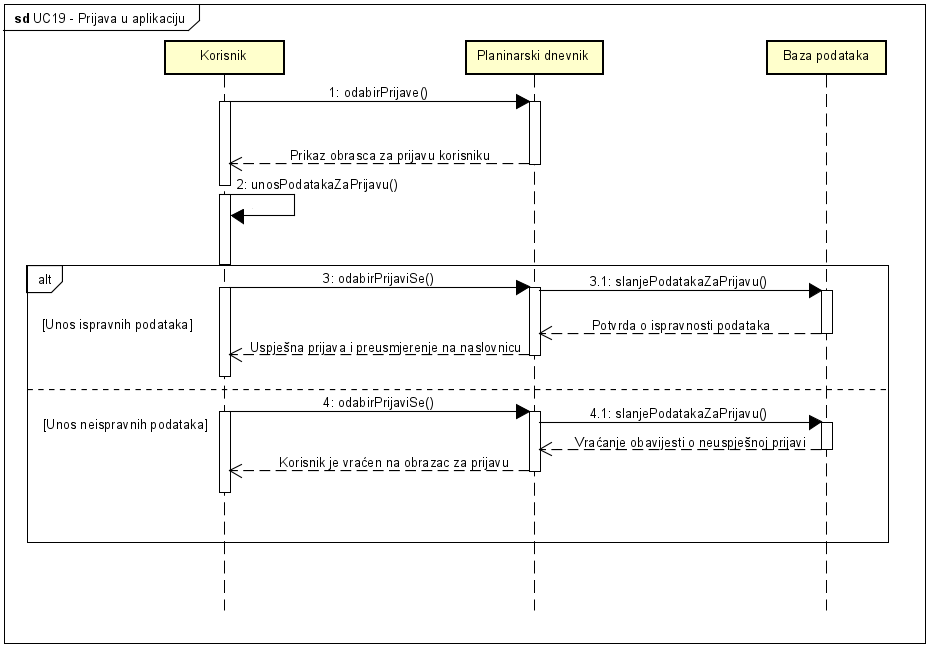
\includegraphics[width=0.9\textwidth]{slike/UC19-Prijava_u_aplikaciju.png}
					\caption{Sekvencijski dijagram za UC19}
						\label{fig:mesh7}
				\end{figure}
				
\newpage
				
				\textbf{ Obrazac uporabe 22 - Promjena osobnih podataka}\\
				
Korisnik je registriran i prijavljen u aplikaciju planinarskog dnevnika te odabire opciju ''osobni podatci''. Baza podataka prikuplja potrebne informacije o korisniku te ih šalje aplikaciji. Korisniku se prikazuju njegovi podatci te mu se pruža mogućnost da ih promijeni. Korisnik može unijeti promjene koje će baza podataka primiti i ažurirati ih te prikazati novo stanje u aplikaciji. Ukoliko korisnik unese nedozvoljene podatke aplikacija ga obavještava te je vraćen na prijašnju stranicu i može vidjeti koji podatci se nisu uspješno ažurirali.				
				
				
				\begin{figure}[H]
					\centering
						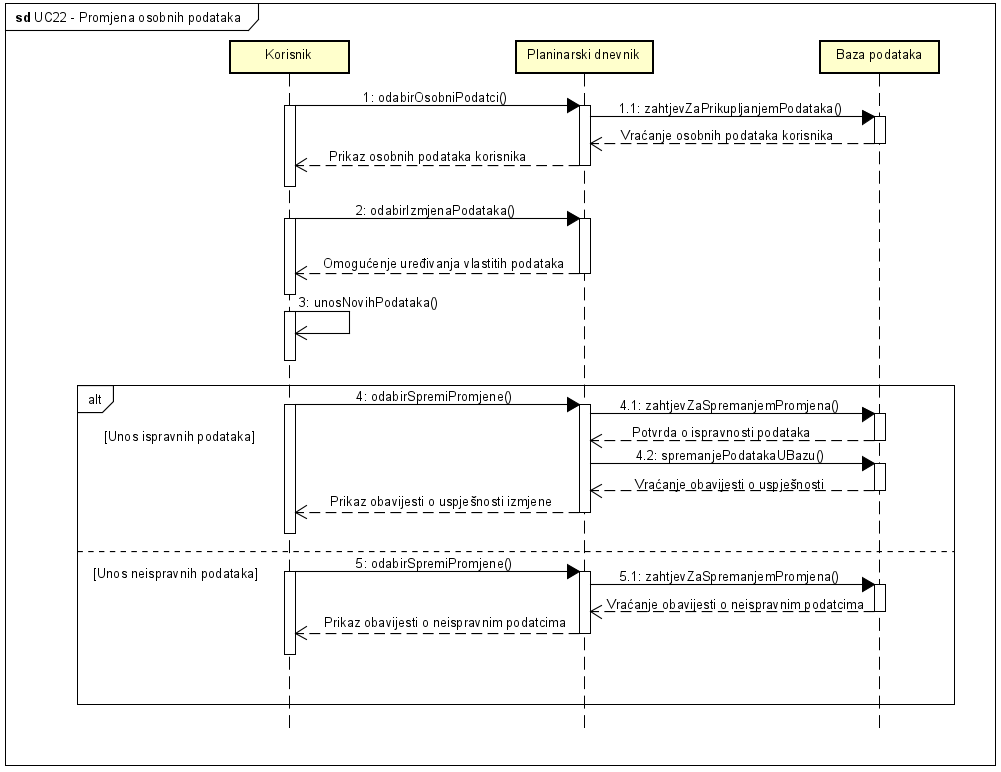
\includegraphics[width=0.9\textwidth]{slike/UC22-Promjena_osobnih_podataka.png}
					\caption{Sekvencijski dijagram za UC22}
						\label{fig:mesh8}
				\end{figure}
	
\newpage
	
\section{Ostali zahtjevi}
\begin{itemize}
	\item Sustav treba omogućiti rad više korisnika u stvarnom vremenu
	\item Korisničko sučelje i sustav moraju podržavati hrvatsku abecedu (dijakritičke znakove) pri unosu i prikazu tekstualnog sadržaja
	\item Izvršavanje dijela programa u kojem se pristupa bazi podataka ne smije trajati duže od nekoliko sekundi
	\item Sustav treba biti implementiran kao web aplikacija koristeći objektno orijentirane jezike
	\item Neispravno korištenje korisničkog sučelja ne smije narušiti funkcionalnost i rad sustava
	\item Sustav treba biti jednostavan za korištenje, korisnici se moraju znati koristiti sučeljem bez opširnih uputa
	\item Nadogradnja sustava ne smije narušavati postojeće funkcionalnosti sustava
	\item Veza s bazom podataka mora biti kvalitetno zaštićena, brza i otporna na vanjske greške 
	\item Dizajn sustava mora biti responzivan, to jest potrebno je omogućiti funkcionalno korištenje na računalu, kao i na tabletu i mobitelu
	\item Pristup sustavu mora biti omogućen iz javne mreže pomoću HTTPS
\end{itemize}
	\chapter{Arhitektura i dizajn sustava}
		
		Arhitektura se može podijeliti na tri podsustava:
		\begin{itemize}
			\item 	\textit{Web aplikacija}
			\item 	\textit{Web poslužitelj}  
			\item 	\textit{Baza podataka}
		\end{itemize}
	
		\textit{\textbf{Web preglednik}} je program koji korisniku omogućuje pregled web-stranica. Svaki internetski  preglednik  je  u suštini prevoditelj, on interpretira programski jezik kojim je stranica napisana te korisniku prikazuje rezultat tog prevođenja. Korisnik  putem  web  preglednika šalje  zahtjev  web poslužitelju.
		
		\textit{\textbf{Web poslužitelj}} je osnova rada web aplikacije. Njegova primarna zadaća je komunikacija klijenta s aplikacijom koja se odvija preko HTTP (engl.HyperText Transfer Protocol) protokola, što je standardni protokol u prijenosu informacija na webu. Poslužitelj je onaj koji pokreće web aplikaciju te joj prosljeđuje zahtjev.
		
		Korisnik koristi web aplikaciju za obrađivanje željenih zahtjeva. Web aplikacija obrađuje zahtjev te, ovisno o zahtjevu, pristupa bazi podataka, nakon čega preko poslužitelja vraća odgovor korisniku, u obliku HTML dokumenta vidljivog u web pregledniku.
		
		Naša web aplikacija je podijeljena na dva glavna dijela: \textit{backend} i \textit{frontend}. Za rad na backendu odlučili smo se za programski jezik Java. Koristimo radni okvir Spring Boot. Java Spring Boot nam nudi unaprijed konfigurirane klase Spring radnog okvira, što nam štedi puno vremena jer se ne moramo zamarati konfiguracijom.\\ \\
		Backend je podijeljen u tri sloja: \textit{controller}, \textit{service} i \textit{repository}. \\ \\
		\begin{figure}[H]
				\centering
				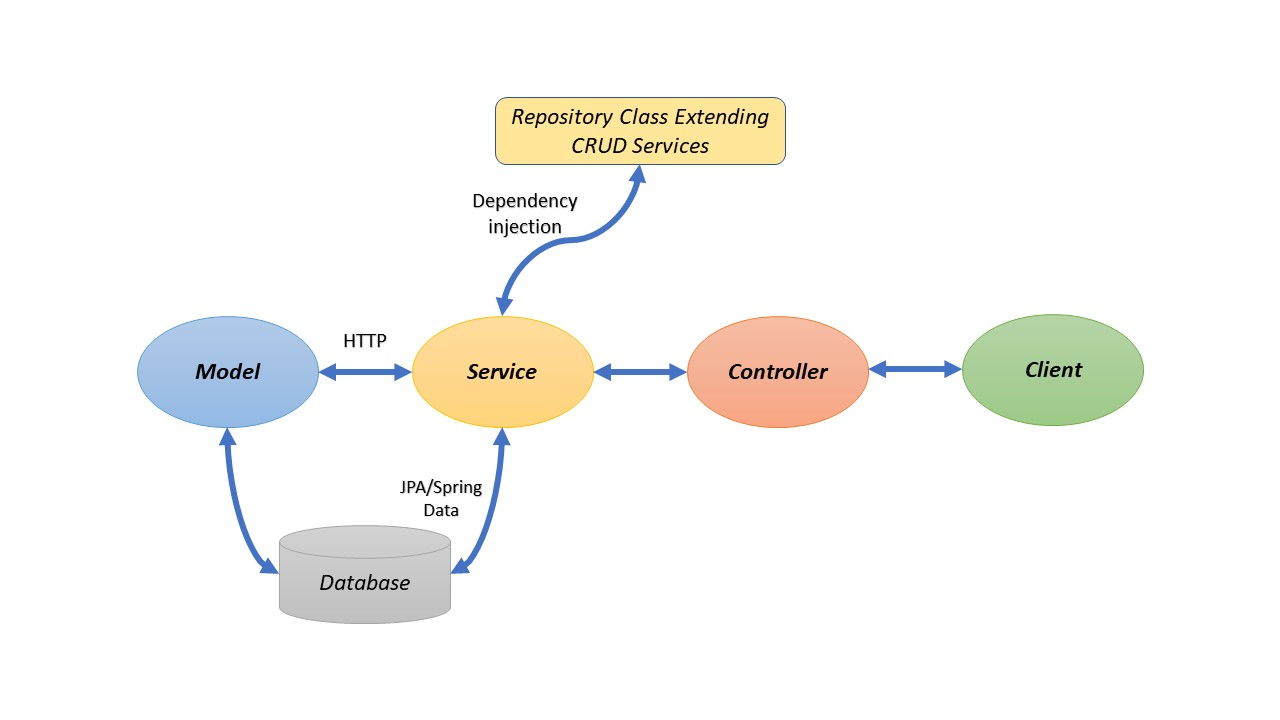
\includegraphics[width=0.9\textwidth]{slike/Spring_dijagram.jpg}
				\caption{Spring dijagram}
				\label{fig:mesh1}
		\end{figure}

		\begin{itemize}
			\item 	\textit{\textit{\textbf{Controller}} komunicira s frontendom  te obrađuje HTTP zahtjeve koje mu frontend pošalje te je u skladu s REST principima.}
			\item 	\textit{\textbf{Service}} sadrži poslovnu logiku aplikacije te je veza između \textit{controllera} i \textit{repositoryja}. On prima podatke iz \textit{controllera} i \textit{repositoryja} te odlučuje što će s tim podacima napraviti (odbaciti, proslijediti, izmijeniti,...) 
			\item 	\textit{\textbf{Repository}} komunicira s bazom podataka te sve zahtjeve prima od servisa i njemu ih vraća.
		\end{itemize}
	
			Uz to koristimo još \textit{entitete} i \textit{DTOs (Data transfer objects)}. DTO je objekt koji se prenosi između procesa. On ne sadrži nikakvu poslovnu logiku, ali može sadržavati mehanizme serijalizacije i deserijalizacije za prijenos podataka.\\ 

			Za rad na frontendu smo se odlučili za \textit{React (JavaScript library)}. Reactov kod se sastoji od entiteta i komponenti. Komponente mogu biti  prikazane u određenom elementu u DOM-u. React je odličan jer se mogu kreirati komponente koje možemo ponovno upotrijebiti bez da pišemo isti/sličan kod na više mjesta.\\
			Razvojno okruženje koje koristimo je InteliJ.

				
		\section{Baza podataka}
			
			Za potrebe naše aplikacije koristit ćemo relacijsku bazu podataka. Baza podataka
			se sastoji od više relacija (takozvanih tablica ili entiteta). Svaka od tih relacija je definirana imenom relacije i skupom atributa koji pobliže opisuju samu relaciju.
			Baza podataka nam služi za pohranu, izmjenu i dohvat potrebnih podataka. Baza
			podataka ove aplikacije sastoji se od sljedećih entiteta:
			\begin{itemize}
				\item 	\textbf{Korisnik}
				\item 	\textbf{Izlet}
				\item 	\textbf{Planinarski dom}
				\item 	\textbf{Geografsko područje}
				\item 	\textbf{Ocjena}
			\end{itemize}
				
		
		
			\subsection{Opis tablica}
			

				\textbf{Korisnik:} Ovaj entitet sadržava sve relevantne informacije o korisniku aplikacije.
				Sadrži sljedeće atribute: jedinstveni identifikator, korisničko ime, lozinku,
				ime, prezime, link za sliku profila, razinu ovlasti korisnika. Ovaj entitet
				je u vezi: \textit{Many-to-Many} s entitetom \textit{Izlet} preko atributa \textit{ID}. Primarni ključ
				entiteta jest atribut \textit{ID}.
				
				\begin{longtabu} to \textwidth {|X[7, l]|X[6, l]|X[21, l]|}
					
					\hline \multicolumn{3}{|c|}{\textbf{Korisnik}}	 \\[3pt] \hline
					\endfirsthead
					
					\hline \multicolumn{3}{|c|}{\textbf{Korisnik}}	 \\[3pt] \hline
					\endhead
					
					\hline 
					\endlastfoot
					
					\cellcolor{LightGreen}ID & BIGINT	&  Jedinstveni identifikator korisnika 	\\ \hline
					Korisničko ime & VARCHAR & Korisničko ime  	\\ \hline 
					Lozinka & VARCHAR & Hash lozinke		\\ \hline 
					Ime & VARCHAR	&  	Ime korisnika			\\ \hline 
					Prezime & VARCHAR	& Prezime korisnika			\\ \hline 
					Slika profila & VARCHAR	&Link za sliku profila		\\ \hline 
					Razina ovlasti& VARCHAR	& Korisnikova uloga		\\ \hline 
			
				\end{longtabu}
			
				\textbf{Izlet:} Ovaj entitet sadržava sve relevantne informacije za jedan izlet.
				Sadrži sljedeće atribute: jedinstveni identifikator, vrh, trajanje, duljinu staze, težinu,
				oznaku o tome je li privatan ili javan i identifikator za ocjenu. Ovaj entitet
				je u vezi: \textit{Many-to-Many} s entitetom \textit{Korisnik} preko atributa \textit{ID}, \textit{Many-to-Many} s entitetom \textit{Planinarski dom} preko atributa \textit{ID},   \textit{Many-to-One} s entitetom \textit{Geografsko područje} preko atributa \textit{ID} i \textit{One-to-Many} s entitetom \textit{Ocjena} preko atributa \textit{ID} . Primarni ključ entiteta jest atribut \textit{ID}.
				
				\begin{longtabu} to \textwidth {|X[7, l]|X[6, l]|X[21, l]|}
					
					\hline \multicolumn{3}{|c|}{\textbf{Izlet}}	 \\[3pt] \hline
					\endfirsthead
					
					\hline \multicolumn{3}{|c|}{\textbf{Izlet}}	 \\[3pt] \hline
					\endhead
					
					\hline 
					\endlastfoot
					
					\cellcolor{LightGreen}ID & BIGINT	&  Jedinstveni identifikator izleta 	\\ \hline
					Vrh				& VARCHAR 	& Naziv vrha izleta  	\\ \hline 
					Trajanje		& BIGINT 	& Vrijeme trajanja izleta		\\ \hline 
					Duljina 		& DECIMAL	& Duljina staze			\\ \hline 
					Težina 			& BIGINT	& Težina staze			\\ \hline 
					Javan			& BOOLEAN	& Oznaka je li izlet javan ili privatan		\\ \hline 
					Ocjena ID		& BIGINT	& Strani ključ koji povezuje relaciju \textit{Izlet}	i \textit{Ocjena}	\\ \hline 
					Područje ID		& BIGINT	& Strani ključ koji povezuje relaciju \textit{Izlet}	i \textit{Geografsko područje}	\\ \hline 
					Opis			& VARCHAR	& Kratki opis izleta		\\ \hline 
					
				\end{longtabu}
			
			
				\textbf{Planinarski dom:} Ovaj entitet sadržava sve relevantne informacije o planinarskom domu.
				Sadrži sljedeće atribute: jedinstveni identifikator, naziv doma, oznaka o prenoćištu, oznaka o hrani, oznaka o vodi i oznaka o struji. Ovaj entitet
				je u vezi: \textit{Many-to-Many} s entitetom \textit{Izlet} preko atributa \textit{ID}, Primarni ključ entiteta jest atribut \textit{ID}.
				
				
				\begin{longtabu} to \textwidth {|X[7, l]|X[6, l]|X[21, l]|}
					
					\hline \multicolumn{3}{|c|}{\textbf{Planinarski dom}}	 \\[3pt] \hline
					\endfirsthead
					
					\hline \multicolumn{3}{|c|}{\textbf{Planinarski dom}}	 \\[3pt] \hline
					\endhead
					
					\hline 
					\endlastfoot
					
					\cellcolor{LightGreen}ID & BIGINT	&  Jedinstveni identifikator planinarskog doma 	\\ \hline
					Naziv			& VARCHAR 	& Naziv planinarskog doma  	\\ \hline 
					Noćenje			& BOOLEAN 	& Oznaka o prenoćištu		\\ \hline 
					Hrana 			& BOOLEAN	& Oznaka o opskrbi hranom			\\ \hline 
					Voda 			& BOOLEAN	& Oznaka o opskrbi vodom			\\ \hline 
					Struja			& BOOLEAN	& Oznaka o dostupnosti struje		\\ \hline 
					
					
				\end{longtabu}
			
			
				\textbf{Geografsko područje:} Ovaj entitet sadržava sve relevantne informacije o geografskom području.
				Sadrži sljedeće atribute: jedinstveni identifikator, naziv područja. Ovaj entitet
				je u vezi: \textit{Many-to-Many} s entitetom \textit{Izlet} preko atributa \textit{ID}, Primarni ključ entiteta jest atribut \textit{ID}.
				
				
				\begin{longtabu} to \textwidth {|X[7, l]|X[6, l]|X[21, l]|}
					
					\hline \multicolumn{3}{|c|}{\textbf{Geografsko područje}}	 \\[3pt] \hline
					\endfirsthead
					
				
					
					\hline 
					\endlastfoot
					
					\cellcolor{LightGreen}ID & BIGINT	&  Jedinstveni identifikator geografskog područja 	\\ \hline
					Naziv			& VARCHAR 	& Naziv geografskog područja 	\\ \hline 
				
					
					
				\end{longtabu}
			
					
				\textbf{Ocjena:} Ovaj entitet sadržava sve relevantne informacije o ocjeni. Sadrži sljedeće atribute: jedinstveni identifikator, ocjena i komentar. Ovaj entitet
				je u vezi: \textit{Many-to-One} s entitetom \textit{Izlet} preko atributa \textit{ID}, Primarni ključ entiteta jest atribut \textit{ID}.
				
				
				\begin{longtabu} to \textwidth {|X[7, l]|X[6, l]|X[21, l]|}
					
					\hline \multicolumn{3}{|c|}{\textbf{Ocjena}}	 \\[3pt] \hline
					\endfirsthead
					
					\hline \multicolumn{3}{|c|}{\textbf{Ocjena}}	 \\[3pt] \hline
					\endhead
					
					\hline 
					\endlastfoot
					
					\cellcolor{LightGreen}ID & BIGINT	&  Jedinstveni identifikator geografskog područja 	\\ \hline
					Ocjena					& BIGINT 	& Predstavlja ocjenu izleta 	\\ \hline 
					Komentar				& VARCHAR 	& Komentar uz ocjenu	\\ \hline 
					
					
				\end{longtabu}
				
			
			
			
			
			
			
			
			
			
			
			
			
			
			
			
			
			
			
			
			
			
			
			
			\subsection{Dijagram baze podataka}
				\begin{figure}[H]
				\centering
				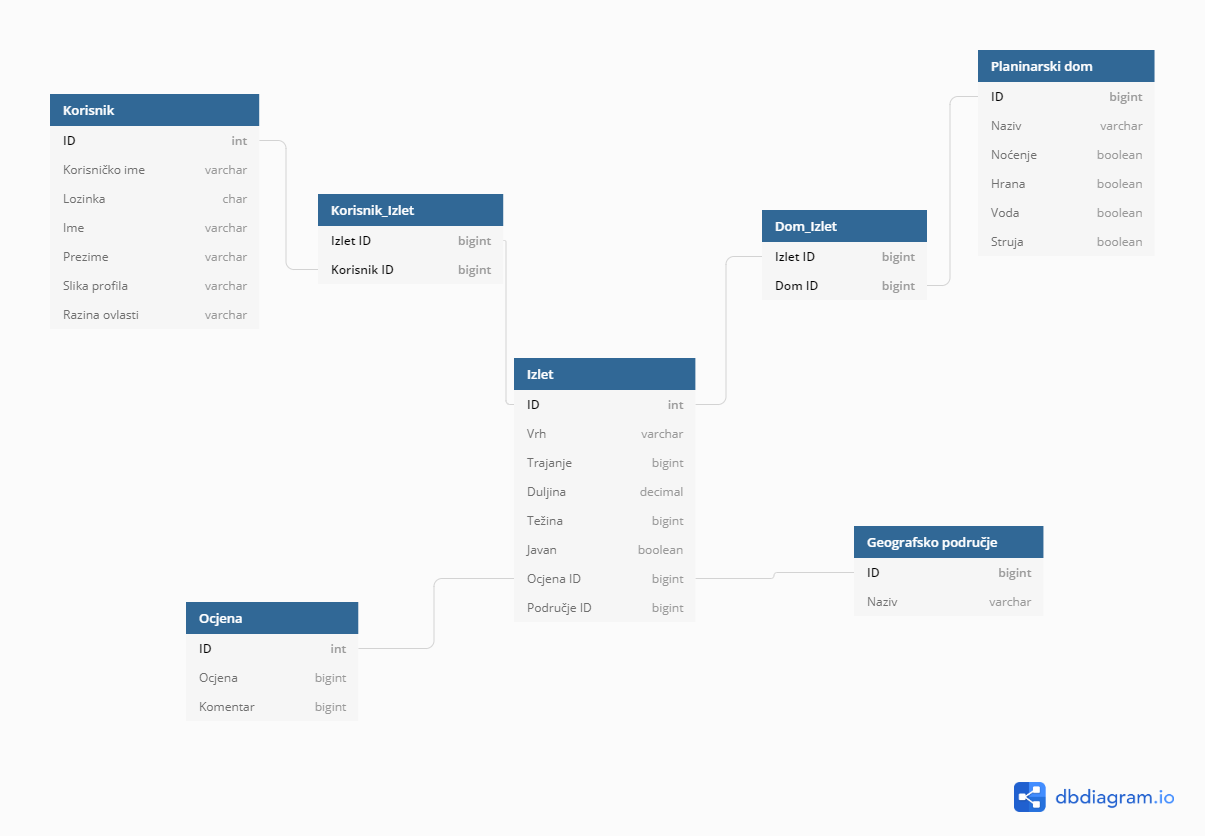
\includegraphics[width=1.1\textwidth]{slike/Baza_dijagram.png}
				\caption{Dijagram baze podataka}
				\label{fig:mesh1}
			\end{figure}
			\eject
			
			
		\section{Dijagram razreda}
			Na slikama: (4.3, 4.4 i 4.5) nalaze se dijagrami razreda. Na dijagramima se nalaze komponente koje opisuju trenutno stanje aplikacije, ali i konceptualni prikaz komponenti koje će se tek pojaviti (npr. \textit{Event, Badge, Administrator...}). U daljnjem radu i razvoju aplikacije doći će do promjena i nadopuna dijagrama razreda. \\
			Dijagrami su podijeljeni u tri cjeline (\textit{Controller, DTO} i \textit{Model}) radi lakšeg snalaženja i preglednosti.
			
			\begin{figure}[H]
				\centering
				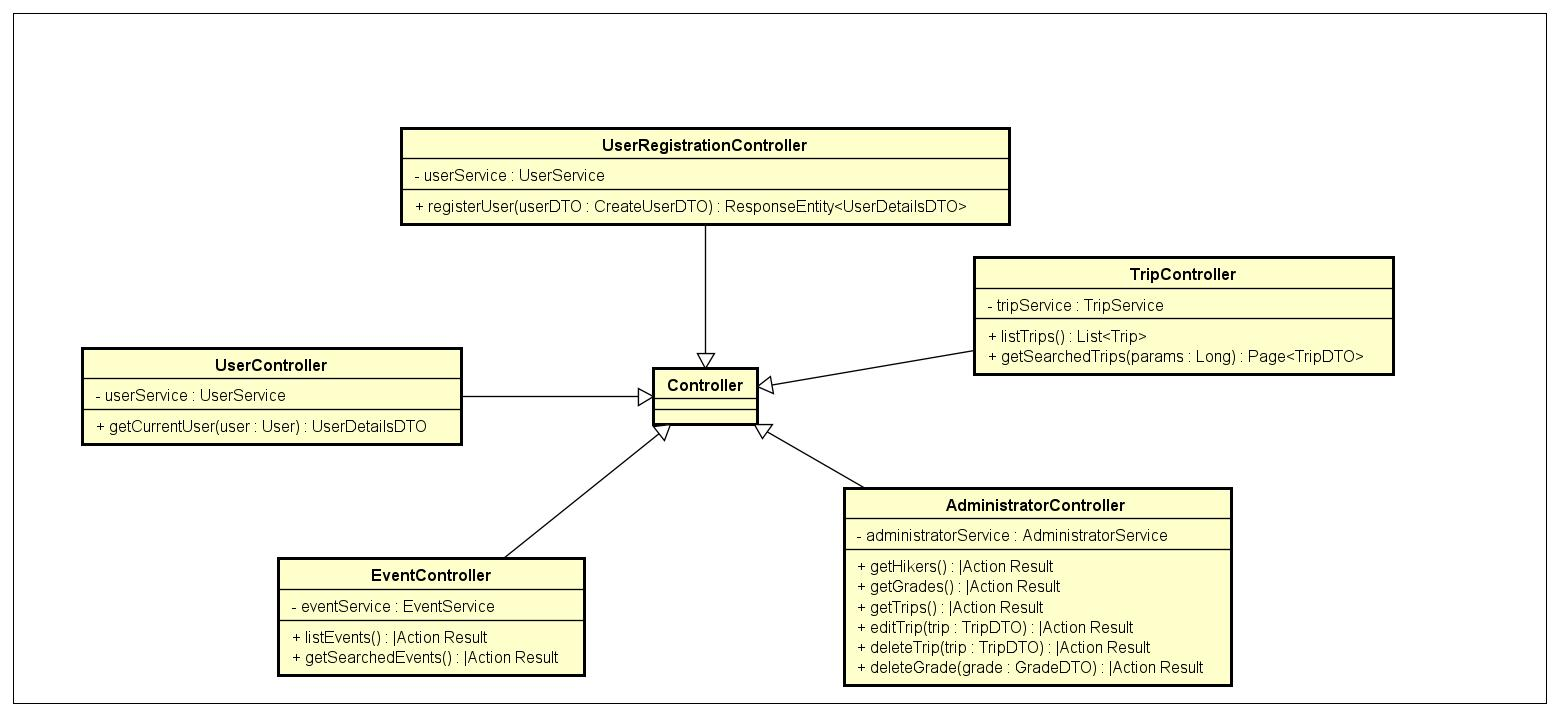
\includegraphics[width=1.1\textwidth]{slike/Controller_dijagram.jpg}
				\caption{Dijagram razreda Controller}
				\label{fig:mesh1}
			\end{figure} 
			
			\begin{figure}[H]
				\centering
				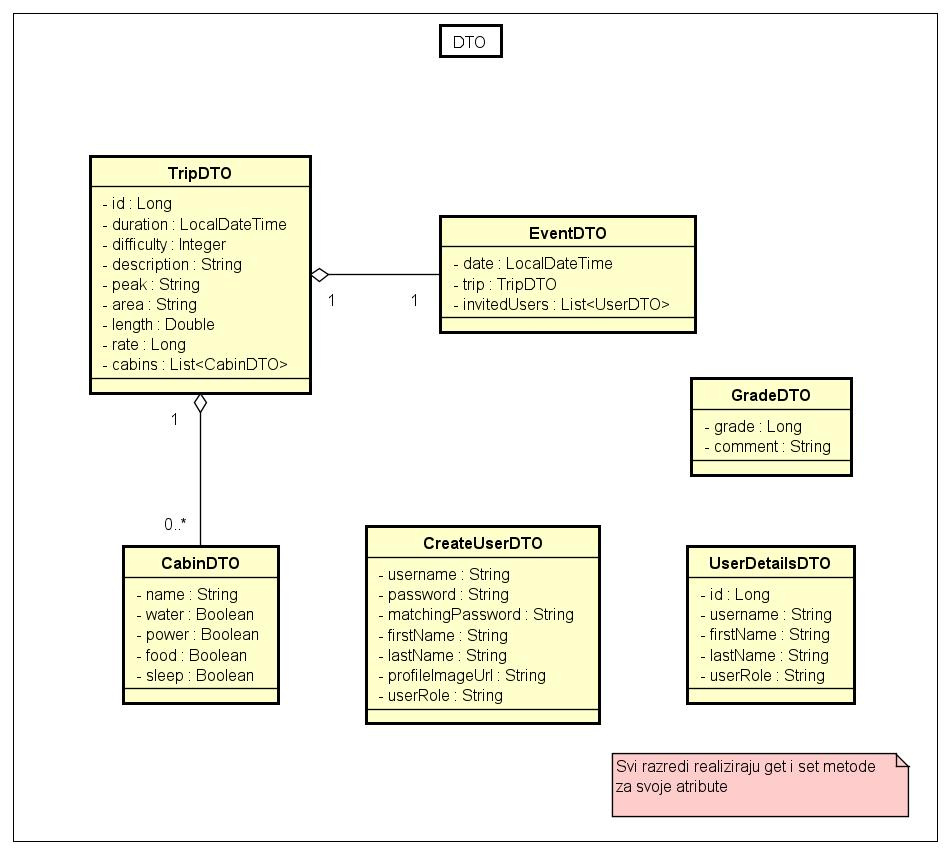
\includegraphics[width=0.9\textwidth]{slike/DTO_dijagram.jpg}
				\caption{Dijagram razreda DTO}
				\label{fig:mesh1}
			\end{figure}
			
			\begin{figure}[H]
				\centering
				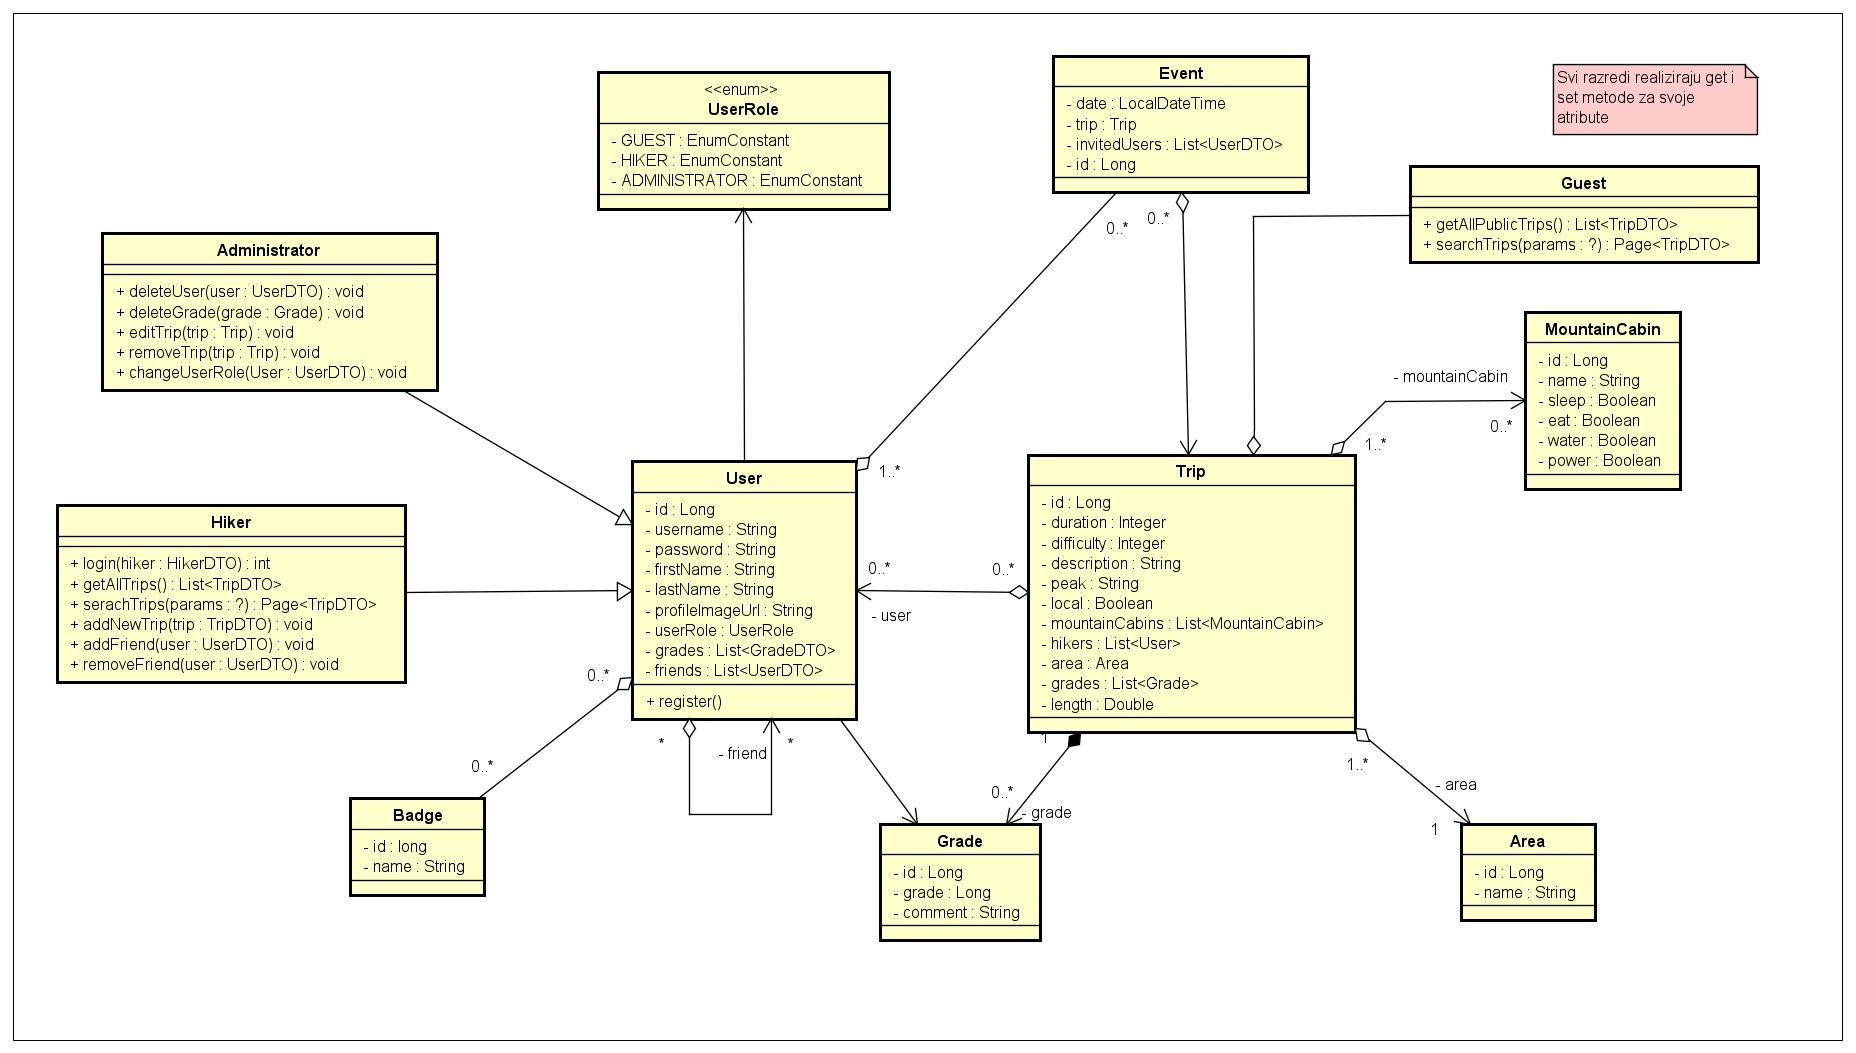
\includegraphics[width=0.9\textwidth]{slike/Model_dijagram.jpg}
				\caption{Dijagram razreda Model}
				\label{fig:mesh1}
			\end{figure} 
			
			\textit{Potrebno je priložiti dijagram razreda s pripadajućim opisom. Zbog preglednosti je moguće dijagram razlomiti na više njih, ali moraju biti grupirani prema sličnim razinama apstrakcije i srodnim funkcionalnostima.}\\
			
			\textbf{\textit{dio 1. revizije}}\\
			
			\textit{Prilikom prve predaje projekta, potrebno je priložiti potpuno razrađen dijagram razreda vezan uz \textbf{generičku funkcionalnost} sustava. Ostale funkcionalnosti trebaju biti idejno razrađene u dijagramu sa sljedećim komponentama: nazivi razreda, nazivi metoda i vrste pristupa metodama (npr. javni, zaštićeni), nazivi atributa razreda, veze i odnosi između razreda.}\\
			
			\textbf{\textit{dio 2. revizije}}\\			
			
			\textit{Prilikom druge predaje projekta dijagram razreda i opisi moraju odgovarati stvarnom stanju implementacije}
			
			
			
			\eject
		
		\section{Dijagram stanja}
			
			
			\textbf{\textit{dio 2. revizije}}\\
			
			\textit{Potrebno je priložiti dijagram stanja i opisati ga. Dovoljan je jedan dijagram stanja koji prikazuje \textbf{značajan dio funkcionalnosti} sustava. Na primjer, stanja korisničkog sučelja i tijek korištenja neke ključne funkcionalnosti jesu značajan dio sustava, a registracija i prijava nisu. }
			
			
			\eject 
		
		\section{Dijagram aktivnosti}
			
			\textbf{\textit{dio 2. revizije}}\\
			
			 \textit{Potrebno je priložiti dijagram aktivnosti s pripadajućim opisom. Dijagram aktivnosti treba prikazivati značajan dio sustava.}
			
			\eject
		\section{Dijagram komponenti}
		
			\textbf{\textit{dio 2. revizije}}\\
		
			 \textit{Potrebno je priložiti dijagram komponenti s pripadajućim opisom. Dijagram komponenti treba prikazivati strukturu cijele aplikacije.}
	\include{Implementacija}
	\include{Zakljucak}
	\include{Literatura}
	
	
	\begingroup
	\renewcommand*\listfigurename{Indeks slika i dijagrama}
	%\renewcommand*\listtablename{Indeks tablica}
	%\let\clearpage\relax
	\listoffigures
	%\vspace{10mm}
	%\listoftables
	\endgroup
	\addcontentsline{toc}{chapter}{Indeks slika i dijagrama}


	
	\eject 
		
	\chapter*{Dodatak: Prikaz aktivnosti grupe}
		\addcontentsline{toc}{chapter}{Dodatak: Prikaz aktivnosti grupe}
		
		\section*{Dnevnik sastajanja}
		
		\textbf{\textit{Kontinuirano osvježavanje}}\\
		
		\begin{packed_enum}
			\item sastanak
			
			\item[] \begin{packed_item}
				\item Datum: 5. listopada 2020.
				\item Prisustvovali: Boltek, Bukovac, Ferković, Kranjčević, Krišković, Pepić, Rožić
				\item Teme sastanka:
				\begin{packed_item}
					\item  upoznavanje, stvaranje ugodne radne atmosfere
					\item  rasprava o eventualnom prijedlogu zadatka
				\end{packed_item}
			\end{packed_item}
			
			\item sastanak
			\item[] \begin{packed_item}
				\item Datum: 9. listopada 2020.
				\item Prisustvovali: Boltek, Bukovac, Ferković, Kranjčević, Krišković, Rožić
				\item Teme sastanka:
				\begin{packed_item}
					\item saznali tko je koliko vješt u kojim tehnologijama
					\item okvirno definirali uloge u ekipi
					\item definirali što ćemo raditi u kojem sprintu
				\end{packed_item}
			\end{packed_item}
		
			\item sastanak
			\item[] \begin{packed_item}
				\item Datum: 15. listopada 2020.
				\item Prisustvovali: Boltek, Bukovac, Ferković, Kranjčević, Krišković, Pepić, Rožić
				\item Teme sastanka:
				\begin{packed_item}
					\item postavili radna okruženja
					\item pomogli onima koji nisu toliko vješti u Gitu, Reactu, Springu, Nodeu i sl. u uspostavljanju radnih okruženja
				\end{packed_item}
			\end{packed_item}
		
			\item sastanak
			\item[] \begin{packed_item}
				\item Datum: 22. listopada 2020.
				\item Prisustvovali: Boltek, Bukovac, Ferković, Kranjčević, Krišković, Pepić, Rožić
				\item Teme sastanka:
				\begin{packed_item}
					\item upoznali se s MVC modelom
					\item zajedno pogledali trenutnu verziju ER modela baze podataka
					\item ukazali na neke trenutne specifičnosti u kodu
				\end{packed_item}
			\end{packed_item}
		
			\item sastanak
			\item[] \begin{packed_item}
				\item Datum: 12. studenog 2020.
				\item Prisustvovali: Boltek, Bukovac, Ferković, Kranjčević, Krišković, Pepić, Rožić
				\item Teme sastanka:
				\begin{packed_item}
					\item prodiskutirali trenutno stanje aplikacije prije prve predaje
					\item prokomentirali daljnje korake vezane uz aplikaciju
					\item sastali se s asistentima te demonstrirali generičke funkcionalnosti
				\end{packed_item}
			\end{packed_item}
			
			%
			
		\end{packed_enum}
		
		\eject
		\section*{Tablica aktivnosti}
		
			\textbf{\textit{Kontinuirano osvježavanje}}\\
			
			 \textit{Napomena: Doprinose u aktivnostima treba navesti u satima po članovima grupe po aktivnosti.}
					
						
			
			\begin{longtabu} to \textwidth {|X[7, l]|X[1, c]|X[1, c]|X[1, c]|X[1, c]|X[1, c]|X[1, c]|X[1, c]|}
								
				\cline{2-8} \multicolumn{1}{c|}{\textbf{}} &     \multicolumn{1}{c|}{\rotatebox{90}{\textbf{Tin Ferković }}} & \multicolumn{1}{c|}{\rotatebox{90}{\textbf{Matej Boltek }}} &	\multicolumn{1}{c|}{\rotatebox{90}{\textbf{Leon Kranjčević }}} &	\multicolumn{1}{c|}{\rotatebox{90}{\textbf{Marko Pepić }}} &
				\multicolumn{1}{c|}{\rotatebox{90}{\textbf{Jakon Dominik Rožić }}} &
				\multicolumn{1}{c|}{\rotatebox{90}{\textbf{Marko Krišković }}} &	\multicolumn{1}{c|}{\rotatebox{90}{\textbf{Antonio Bukovac }}} \\ \hline 
				\endfirsthead
				
			
				\cline{2-8} \multicolumn{1}{c|}{\textbf{}} &     \multicolumn{1}{c|}{\rotatebox{90}{\textbf{Tin Ferković}}} & \multicolumn{1}{c|}{\rotatebox{90}{\textbf{Matej Boltek }}} &	\multicolumn{1}{c|}{\rotatebox{90}{\textbf{Leon Kranjčević }}} &
				\multicolumn{1}{c|}{\rotatebox{90}{\textbf{Marko Pepić }}} &	\multicolumn{1}{c|}{\rotatebox{90}{\textbf{Jakov Dominik Rožić }}} &
				\multicolumn{1}{c|}{\rotatebox{90}{\textbf{Marko Krišković }}} &	\multicolumn{1}{c|}{\rotatebox{90}{\textbf{Antonio Bukovac }}} \\ \hline 
				\endhead
				
				
				\endfoot
							
				 
				\endlastfoot
				
				Upravljanje projektom 		&5  &  &2  &  & 1 &  &1 \\ \hline
				Opis projektnog zadatka 	&1  &  &4 & 6 & 2 & 1 &1 \\ \hline
				Funkcionalni zahtjevi       &  & 1 & 1 & 1 & 2 & 5 &  \\ \hline
				Dijagram obrazaca 			&3  & 1 & 1 & 4 & 5 & 2 &4  \\ \hline
				Opis ostalih zahtjeva 		&  & 2 &1  &1  & 1 & 1 &1  \\ \hline
				Opis pojedinih obrazaca 	&3  & 3 &1 & 2 & 6 & 1 &4  \\ \hline
				Sekvencijski dijagrami 		&1  & 1 &1  & 1 & 3 &  &1  \\ \hline
				Arhitektura i dizajn sustava	 &4  & 2 &5  & 3 & 1 &  &5  \\ \hline
				Baza podataka				&2  & 2 &3  & 1 &  & 2 &3   \\ \hline
				Dijagram razreda 			&1  & 1 &2  & 2 & 3 & 1 &3   \\ \hline
				Dijagram stanja				&  &  &  &  &  &  &  \\ \hline
				Dijagram aktivnosti 		&  &  &  &  &  &  &  \\ \hline
				Dijagram komponenti			&  &  &  &  &  &  &  \\ \hline
				Korištene tehnologije i alati 		&  &  &  &  &  &  &  \\ \hline
				Ispitivanje programskog rješenja 	&  &  &  &  &  &  &  \\ \hline
				Dijagram razmještaja			&  &  &  &  &  &  &  \\ \hline
				Upute za puštanje u pogon 		&  &  &  &  &  &  &  \\ \hline 
				Dnevnik sastajanja 			&1  &  &  &  &  &  &  \\ \hline
				Zaključak i budući rad 		&  &  &  &  &  &  &  \\  \hline
				Popis literature 			&  &  &  &  &  &  &  \\  \hline
				Prijava u aplikaciju 			&2  & 1 & 4 & 2 & 1 & 2 & 2 \\ \hline
				Registracija u aplikaciju 				&2  & 4 &1 &1  & 1 & 2 &  \\ \hline 
				Filter izleta 		 			&3  &  &5  &1  &  & 5 & 2 \\ \hline 
				Zaglavlje aplikacije 							& 1 &4  &  &  &  &  &  \\ \hline

				
				
				
			\end{longtabu}
					
					
		\eject
		\section*{Dijagrami pregleda promjena}
		
		\textbf{\textit{dio 2. revizije}}\\
		
		\textit{Prenijeti dijagram pregleda promjena nad datotekama projekta. Potrebno je na kraju projekta generirane grafove s gitlaba prenijeti u ovo poglavlje dokumentacije. Dijagrami za vlastiti projekt se mogu preuzeti s gitlab.com stranice, u izborniku Repository, pritiskom na stavku Contributors.}
		
	


\end{document} %naredbe i tekst nakon ove naredbe ne ulaze u izgrađen dokument 
